
    




    
\documentclass[11pt]{article}

    
    \usepackage[breakable]{tcolorbox}
    \tcbset{nobeforeafter} % prevents tcolorboxes being placing in paragraphs
    \usepackage{float}
    \floatplacement{figure}{H} % forces figures to be placed at the correct location
    
    \usepackage[T1]{fontenc}
    % Nicer default font (+ math font) than Computer Modern for most use cases
    \usepackage{mathpazo}

    % Basic figure setup, for now with no caption control since it's done
    % automatically by Pandoc (which extracts ![](path) syntax from Markdown).
    \usepackage{graphicx}
    % We will generate all images so they have a width \maxwidth. This means
    % that they will get their normal width if they fit onto the page, but
    % are scaled down if they would overflow the margins.
    \makeatletter
    \def\maxwidth{\ifdim\Gin@nat@width>\linewidth\linewidth
    \else\Gin@nat@width\fi}
    \makeatother
    \let\Oldincludegraphics\includegraphics
    % Set max figure width to be 80% of text width, for now hardcoded.
    \renewcommand{\includegraphics}[1]{\Oldincludegraphics[width=.8\maxwidth]{#1}}
    % Ensure that by default, figures have no caption (until we provide a
    % proper Figure object with a Caption API and a way to capture that
    % in the conversion process - todo).
    \usepackage{caption}
    \DeclareCaptionLabelFormat{nolabel}{}
    \captionsetup{labelformat=nolabel}

    \usepackage{adjustbox} % Used to constrain images to a maximum size 
    \usepackage{xcolor} % Allow colors to be defined
    \usepackage{enumerate} % Needed for markdown enumerations to work
    \usepackage{geometry} % Used to adjust the document margins
    \usepackage{amsmath} % Equations
    \usepackage{amssymb} % Equations
    \usepackage{textcomp} % defines textquotesingle
    % Hack from http://tex.stackexchange.com/a/47451/13684:
    \AtBeginDocument{%
        \def\PYZsq{\textquotesingle}% Upright quotes in Pygmentized code
    }
    \usepackage{upquote} % Upright quotes for verbatim code
    \usepackage{eurosym} % defines \euro
    \usepackage[mathletters]{ucs} % Extended unicode (utf-8) support
    \usepackage[utf8x]{inputenc} % Allow utf-8 characters in the tex document
    \usepackage{fancyvrb} % verbatim replacement that allows latex
    \usepackage{grffile} % extends the file name processing of package graphics 
                         % to support a larger range 
    % The hyperref package gives us a pdf with properly built
    % internal navigation ('pdf bookmarks' for the table of contents,
    % internal cross-reference links, web links for URLs, etc.)
    \usepackage{hyperref}
    \usepackage{longtable} % longtable support required by pandoc >1.10
    \usepackage{booktabs}  % table support for pandoc > 1.12.2
    \usepackage[inline]{enumitem} % IRkernel/repr support (it uses the enumerate* environment)
    \usepackage[normalem]{ulem} % ulem is needed to support strikethroughs (\sout)
                                % normalem makes italics be italics, not underlines
    \usepackage{mathrsfs}
    

    
    % Colors for the hyperref package
    \definecolor{urlcolor}{rgb}{0,.145,.698}
    \definecolor{linkcolor}{rgb}{.71,0.21,0.01}
    \definecolor{citecolor}{rgb}{.12,.54,.11}

    % ANSI colors
    \definecolor{ansi-black}{HTML}{3E424D}
    \definecolor{ansi-black-intense}{HTML}{282C36}
    \definecolor{ansi-red}{HTML}{E75C58}
    \definecolor{ansi-red-intense}{HTML}{B22B31}
    \definecolor{ansi-green}{HTML}{00A250}
    \definecolor{ansi-green-intense}{HTML}{007427}
    \definecolor{ansi-yellow}{HTML}{DDB62B}
    \definecolor{ansi-yellow-intense}{HTML}{B27D12}
    \definecolor{ansi-blue}{HTML}{208FFB}
    \definecolor{ansi-blue-intense}{HTML}{0065CA}
    \definecolor{ansi-magenta}{HTML}{D160C4}
    \definecolor{ansi-magenta-intense}{HTML}{A03196}
    \definecolor{ansi-cyan}{HTML}{60C6C8}
    \definecolor{ansi-cyan-intense}{HTML}{258F8F}
    \definecolor{ansi-white}{HTML}{C5C1B4}
    \definecolor{ansi-white-intense}{HTML}{A1A6B2}
    \definecolor{ansi-default-inverse-fg}{HTML}{FFFFFF}
    \definecolor{ansi-default-inverse-bg}{HTML}{000000}

    % commands and environments needed by pandoc snippets
    % extracted from the output of `pandoc -s`
    \providecommand{\tightlist}{%
      \setlength{\itemsep}{0pt}\setlength{\parskip}{0pt}}
    \DefineVerbatimEnvironment{Highlighting}{Verbatim}{commandchars=\\\{\}}
    % Add ',fontsize=\small' for more characters per line
    \newenvironment{Shaded}{}{}
    \newcommand{\KeywordTok}[1]{\textcolor[rgb]{0.00,0.44,0.13}{\textbf{{#1}}}}
    \newcommand{\DataTypeTok}[1]{\textcolor[rgb]{0.56,0.13,0.00}{{#1}}}
    \newcommand{\DecValTok}[1]{\textcolor[rgb]{0.25,0.63,0.44}{{#1}}}
    \newcommand{\BaseNTok}[1]{\textcolor[rgb]{0.25,0.63,0.44}{{#1}}}
    \newcommand{\FloatTok}[1]{\textcolor[rgb]{0.25,0.63,0.44}{{#1}}}
    \newcommand{\CharTok}[1]{\textcolor[rgb]{0.25,0.44,0.63}{{#1}}}
    \newcommand{\StringTok}[1]{\textcolor[rgb]{0.25,0.44,0.63}{{#1}}}
    \newcommand{\CommentTok}[1]{\textcolor[rgb]{0.38,0.63,0.69}{\textit{{#1}}}}
    \newcommand{\OtherTok}[1]{\textcolor[rgb]{0.00,0.44,0.13}{{#1}}}
    \newcommand{\AlertTok}[1]{\textcolor[rgb]{1.00,0.00,0.00}{\textbf{{#1}}}}
    \newcommand{\FunctionTok}[1]{\textcolor[rgb]{0.02,0.16,0.49}{{#1}}}
    \newcommand{\RegionMarkerTok}[1]{{#1}}
    \newcommand{\ErrorTok}[1]{\textcolor[rgb]{1.00,0.00,0.00}{\textbf{{#1}}}}
    \newcommand{\NormalTok}[1]{{#1}}
    
    % Additional commands for more recent versions of Pandoc
    \newcommand{\ConstantTok}[1]{\textcolor[rgb]{0.53,0.00,0.00}{{#1}}}
    \newcommand{\SpecialCharTok}[1]{\textcolor[rgb]{0.25,0.44,0.63}{{#1}}}
    \newcommand{\VerbatimStringTok}[1]{\textcolor[rgb]{0.25,0.44,0.63}{{#1}}}
    \newcommand{\SpecialStringTok}[1]{\textcolor[rgb]{0.73,0.40,0.53}{{#1}}}
    \newcommand{\ImportTok}[1]{{#1}}
    \newcommand{\DocumentationTok}[1]{\textcolor[rgb]{0.73,0.13,0.13}{\textit{{#1}}}}
    \newcommand{\AnnotationTok}[1]{\textcolor[rgb]{0.38,0.63,0.69}{\textbf{\textit{{#1}}}}}
    \newcommand{\CommentVarTok}[1]{\textcolor[rgb]{0.38,0.63,0.69}{\textbf{\textit{{#1}}}}}
    \newcommand{\VariableTok}[1]{\textcolor[rgb]{0.10,0.09,0.49}{{#1}}}
    \newcommand{\ControlFlowTok}[1]{\textcolor[rgb]{0.00,0.44,0.13}{\textbf{{#1}}}}
    \newcommand{\OperatorTok}[1]{\textcolor[rgb]{0.40,0.40,0.40}{{#1}}}
    \newcommand{\BuiltInTok}[1]{{#1}}
    \newcommand{\ExtensionTok}[1]{{#1}}
    \newcommand{\PreprocessorTok}[1]{\textcolor[rgb]{0.74,0.48,0.00}{{#1}}}
    \newcommand{\AttributeTok}[1]{\textcolor[rgb]{0.49,0.56,0.16}{{#1}}}
    \newcommand{\InformationTok}[1]{\textcolor[rgb]{0.38,0.63,0.69}{\textbf{\textit{{#1}}}}}
    \newcommand{\WarningTok}[1]{\textcolor[rgb]{0.38,0.63,0.69}{\textbf{\textit{{#1}}}}}
    
    
    % Define a nice break command that doesn't care if a line doesn't already
    % exist.
    \def\br{\hspace*{\fill} \\* }
    % Math Jax compatibility definitions
    \def\gt{>}
    \def\lt{<}
    \let\Oldtex\TeX
    \let\Oldlatex\LaTeX
    \renewcommand{\TeX}{\textrm{\Oldtex}}
    \renewcommand{\LaTeX}{\textrm{\Oldlatex}}
    % Document parameters
    % Document title
    \title{linear\_algebra\_background}
    
    
    
    
    
% Pygments definitions
\makeatletter
\def\PY@reset{\let\PY@it=\relax \let\PY@bf=\relax%
    \let\PY@ul=\relax \let\PY@tc=\relax%
    \let\PY@bc=\relax \let\PY@ff=\relax}
\def\PY@tok#1{\csname PY@tok@#1\endcsname}
\def\PY@toks#1+{\ifx\relax#1\empty\else%
    \PY@tok{#1}\expandafter\PY@toks\fi}
\def\PY@do#1{\PY@bc{\PY@tc{\PY@ul{%
    \PY@it{\PY@bf{\PY@ff{#1}}}}}}}
\def\PY#1#2{\PY@reset\PY@toks#1+\relax+\PY@do{#2}}

\expandafter\def\csname PY@tok@w\endcsname{\def\PY@tc##1{\textcolor[rgb]{0.73,0.73,0.73}{##1}}}
\expandafter\def\csname PY@tok@c\endcsname{\let\PY@it=\textit\def\PY@tc##1{\textcolor[rgb]{0.25,0.50,0.50}{##1}}}
\expandafter\def\csname PY@tok@cp\endcsname{\def\PY@tc##1{\textcolor[rgb]{0.74,0.48,0.00}{##1}}}
\expandafter\def\csname PY@tok@k\endcsname{\let\PY@bf=\textbf\def\PY@tc##1{\textcolor[rgb]{0.00,0.50,0.00}{##1}}}
\expandafter\def\csname PY@tok@kp\endcsname{\def\PY@tc##1{\textcolor[rgb]{0.00,0.50,0.00}{##1}}}
\expandafter\def\csname PY@tok@kt\endcsname{\def\PY@tc##1{\textcolor[rgb]{0.69,0.00,0.25}{##1}}}
\expandafter\def\csname PY@tok@o\endcsname{\def\PY@tc##1{\textcolor[rgb]{0.40,0.40,0.40}{##1}}}
\expandafter\def\csname PY@tok@ow\endcsname{\let\PY@bf=\textbf\def\PY@tc##1{\textcolor[rgb]{0.67,0.13,1.00}{##1}}}
\expandafter\def\csname PY@tok@nb\endcsname{\def\PY@tc##1{\textcolor[rgb]{0.00,0.50,0.00}{##1}}}
\expandafter\def\csname PY@tok@nf\endcsname{\def\PY@tc##1{\textcolor[rgb]{0.00,0.00,1.00}{##1}}}
\expandafter\def\csname PY@tok@nc\endcsname{\let\PY@bf=\textbf\def\PY@tc##1{\textcolor[rgb]{0.00,0.00,1.00}{##1}}}
\expandafter\def\csname PY@tok@nn\endcsname{\let\PY@bf=\textbf\def\PY@tc##1{\textcolor[rgb]{0.00,0.00,1.00}{##1}}}
\expandafter\def\csname PY@tok@ne\endcsname{\let\PY@bf=\textbf\def\PY@tc##1{\textcolor[rgb]{0.82,0.25,0.23}{##1}}}
\expandafter\def\csname PY@tok@nv\endcsname{\def\PY@tc##1{\textcolor[rgb]{0.10,0.09,0.49}{##1}}}
\expandafter\def\csname PY@tok@no\endcsname{\def\PY@tc##1{\textcolor[rgb]{0.53,0.00,0.00}{##1}}}
\expandafter\def\csname PY@tok@nl\endcsname{\def\PY@tc##1{\textcolor[rgb]{0.63,0.63,0.00}{##1}}}
\expandafter\def\csname PY@tok@ni\endcsname{\let\PY@bf=\textbf\def\PY@tc##1{\textcolor[rgb]{0.60,0.60,0.60}{##1}}}
\expandafter\def\csname PY@tok@na\endcsname{\def\PY@tc##1{\textcolor[rgb]{0.49,0.56,0.16}{##1}}}
\expandafter\def\csname PY@tok@nt\endcsname{\let\PY@bf=\textbf\def\PY@tc##1{\textcolor[rgb]{0.00,0.50,0.00}{##1}}}
\expandafter\def\csname PY@tok@nd\endcsname{\def\PY@tc##1{\textcolor[rgb]{0.67,0.13,1.00}{##1}}}
\expandafter\def\csname PY@tok@s\endcsname{\def\PY@tc##1{\textcolor[rgb]{0.73,0.13,0.13}{##1}}}
\expandafter\def\csname PY@tok@sd\endcsname{\let\PY@it=\textit\def\PY@tc##1{\textcolor[rgb]{0.73,0.13,0.13}{##1}}}
\expandafter\def\csname PY@tok@si\endcsname{\let\PY@bf=\textbf\def\PY@tc##1{\textcolor[rgb]{0.73,0.40,0.53}{##1}}}
\expandafter\def\csname PY@tok@se\endcsname{\let\PY@bf=\textbf\def\PY@tc##1{\textcolor[rgb]{0.73,0.40,0.13}{##1}}}
\expandafter\def\csname PY@tok@sr\endcsname{\def\PY@tc##1{\textcolor[rgb]{0.73,0.40,0.53}{##1}}}
\expandafter\def\csname PY@tok@ss\endcsname{\def\PY@tc##1{\textcolor[rgb]{0.10,0.09,0.49}{##1}}}
\expandafter\def\csname PY@tok@sx\endcsname{\def\PY@tc##1{\textcolor[rgb]{0.00,0.50,0.00}{##1}}}
\expandafter\def\csname PY@tok@m\endcsname{\def\PY@tc##1{\textcolor[rgb]{0.40,0.40,0.40}{##1}}}
\expandafter\def\csname PY@tok@gh\endcsname{\let\PY@bf=\textbf\def\PY@tc##1{\textcolor[rgb]{0.00,0.00,0.50}{##1}}}
\expandafter\def\csname PY@tok@gu\endcsname{\let\PY@bf=\textbf\def\PY@tc##1{\textcolor[rgb]{0.50,0.00,0.50}{##1}}}
\expandafter\def\csname PY@tok@gd\endcsname{\def\PY@tc##1{\textcolor[rgb]{0.63,0.00,0.00}{##1}}}
\expandafter\def\csname PY@tok@gi\endcsname{\def\PY@tc##1{\textcolor[rgb]{0.00,0.63,0.00}{##1}}}
\expandafter\def\csname PY@tok@gr\endcsname{\def\PY@tc##1{\textcolor[rgb]{1.00,0.00,0.00}{##1}}}
\expandafter\def\csname PY@tok@ge\endcsname{\let\PY@it=\textit}
\expandafter\def\csname PY@tok@gs\endcsname{\let\PY@bf=\textbf}
\expandafter\def\csname PY@tok@gp\endcsname{\let\PY@bf=\textbf\def\PY@tc##1{\textcolor[rgb]{0.00,0.00,0.50}{##1}}}
\expandafter\def\csname PY@tok@go\endcsname{\def\PY@tc##1{\textcolor[rgb]{0.53,0.53,0.53}{##1}}}
\expandafter\def\csname PY@tok@gt\endcsname{\def\PY@tc##1{\textcolor[rgb]{0.00,0.27,0.87}{##1}}}
\expandafter\def\csname PY@tok@err\endcsname{\def\PY@bc##1{\setlength{\fboxsep}{0pt}\fcolorbox[rgb]{1.00,0.00,0.00}{1,1,1}{\strut ##1}}}
\expandafter\def\csname PY@tok@kc\endcsname{\let\PY@bf=\textbf\def\PY@tc##1{\textcolor[rgb]{0.00,0.50,0.00}{##1}}}
\expandafter\def\csname PY@tok@kd\endcsname{\let\PY@bf=\textbf\def\PY@tc##1{\textcolor[rgb]{0.00,0.50,0.00}{##1}}}
\expandafter\def\csname PY@tok@kn\endcsname{\let\PY@bf=\textbf\def\PY@tc##1{\textcolor[rgb]{0.00,0.50,0.00}{##1}}}
\expandafter\def\csname PY@tok@kr\endcsname{\let\PY@bf=\textbf\def\PY@tc##1{\textcolor[rgb]{0.00,0.50,0.00}{##1}}}
\expandafter\def\csname PY@tok@bp\endcsname{\def\PY@tc##1{\textcolor[rgb]{0.00,0.50,0.00}{##1}}}
\expandafter\def\csname PY@tok@fm\endcsname{\def\PY@tc##1{\textcolor[rgb]{0.00,0.00,1.00}{##1}}}
\expandafter\def\csname PY@tok@vc\endcsname{\def\PY@tc##1{\textcolor[rgb]{0.10,0.09,0.49}{##1}}}
\expandafter\def\csname PY@tok@vg\endcsname{\def\PY@tc##1{\textcolor[rgb]{0.10,0.09,0.49}{##1}}}
\expandafter\def\csname PY@tok@vi\endcsname{\def\PY@tc##1{\textcolor[rgb]{0.10,0.09,0.49}{##1}}}
\expandafter\def\csname PY@tok@vm\endcsname{\def\PY@tc##1{\textcolor[rgb]{0.10,0.09,0.49}{##1}}}
\expandafter\def\csname PY@tok@sa\endcsname{\def\PY@tc##1{\textcolor[rgb]{0.73,0.13,0.13}{##1}}}
\expandafter\def\csname PY@tok@sb\endcsname{\def\PY@tc##1{\textcolor[rgb]{0.73,0.13,0.13}{##1}}}
\expandafter\def\csname PY@tok@sc\endcsname{\def\PY@tc##1{\textcolor[rgb]{0.73,0.13,0.13}{##1}}}
\expandafter\def\csname PY@tok@dl\endcsname{\def\PY@tc##1{\textcolor[rgb]{0.73,0.13,0.13}{##1}}}
\expandafter\def\csname PY@tok@s2\endcsname{\def\PY@tc##1{\textcolor[rgb]{0.73,0.13,0.13}{##1}}}
\expandafter\def\csname PY@tok@sh\endcsname{\def\PY@tc##1{\textcolor[rgb]{0.73,0.13,0.13}{##1}}}
\expandafter\def\csname PY@tok@s1\endcsname{\def\PY@tc##1{\textcolor[rgb]{0.73,0.13,0.13}{##1}}}
\expandafter\def\csname PY@tok@mb\endcsname{\def\PY@tc##1{\textcolor[rgb]{0.40,0.40,0.40}{##1}}}
\expandafter\def\csname PY@tok@mf\endcsname{\def\PY@tc##1{\textcolor[rgb]{0.40,0.40,0.40}{##1}}}
\expandafter\def\csname PY@tok@mh\endcsname{\def\PY@tc##1{\textcolor[rgb]{0.40,0.40,0.40}{##1}}}
\expandafter\def\csname PY@tok@mi\endcsname{\def\PY@tc##1{\textcolor[rgb]{0.40,0.40,0.40}{##1}}}
\expandafter\def\csname PY@tok@il\endcsname{\def\PY@tc##1{\textcolor[rgb]{0.40,0.40,0.40}{##1}}}
\expandafter\def\csname PY@tok@mo\endcsname{\def\PY@tc##1{\textcolor[rgb]{0.40,0.40,0.40}{##1}}}
\expandafter\def\csname PY@tok@ch\endcsname{\let\PY@it=\textit\def\PY@tc##1{\textcolor[rgb]{0.25,0.50,0.50}{##1}}}
\expandafter\def\csname PY@tok@cm\endcsname{\let\PY@it=\textit\def\PY@tc##1{\textcolor[rgb]{0.25,0.50,0.50}{##1}}}
\expandafter\def\csname PY@tok@cpf\endcsname{\let\PY@it=\textit\def\PY@tc##1{\textcolor[rgb]{0.25,0.50,0.50}{##1}}}
\expandafter\def\csname PY@tok@c1\endcsname{\let\PY@it=\textit\def\PY@tc##1{\textcolor[rgb]{0.25,0.50,0.50}{##1}}}
\expandafter\def\csname PY@tok@cs\endcsname{\let\PY@it=\textit\def\PY@tc##1{\textcolor[rgb]{0.25,0.50,0.50}{##1}}}

\def\PYZbs{\char`\\}
\def\PYZus{\char`\_}
\def\PYZob{\char`\{}
\def\PYZcb{\char`\}}
\def\PYZca{\char`\^}
\def\PYZam{\char`\&}
\def\PYZlt{\char`\<}
\def\PYZgt{\char`\>}
\def\PYZsh{\char`\#}
\def\PYZpc{\char`\%}
\def\PYZdl{\char`\$}
\def\PYZhy{\char`\-}
\def\PYZsq{\char`\'}
\def\PYZdq{\char`\"}
\def\PYZti{\char`\~}
% for compatibility with earlier versions
\def\PYZat{@}
\def\PYZlb{[}
\def\PYZrb{]}
\makeatother


    % For linebreaks inside Verbatim environment from package fancyvrb. 
    \makeatletter
        \newbox\Wrappedcontinuationbox 
        \newbox\Wrappedvisiblespacebox 
        \newcommand*\Wrappedvisiblespace {\textcolor{red}{\textvisiblespace}} 
        \newcommand*\Wrappedcontinuationsymbol {\textcolor{red}{\llap{\tiny$\m@th\hookrightarrow$}}} 
        \newcommand*\Wrappedcontinuationindent {3ex } 
        \newcommand*\Wrappedafterbreak {\kern\Wrappedcontinuationindent\copy\Wrappedcontinuationbox} 
        % Take advantage of the already applied Pygments mark-up to insert 
        % potential linebreaks for TeX processing. 
        %        {, <, #, %, $, ' and ": go to next line. 
        %        _, }, ^, &, >, - and ~: stay at end of broken line. 
        % Use of \textquotesingle for straight quote. 
        \newcommand*\Wrappedbreaksatspecials {% 
            \def\PYGZus{\discretionary{\char`\_}{\Wrappedafterbreak}{\char`\_}}% 
            \def\PYGZob{\discretionary{}{\Wrappedafterbreak\char`\{}{\char`\{}}% 
            \def\PYGZcb{\discretionary{\char`\}}{\Wrappedafterbreak}{\char`\}}}% 
            \def\PYGZca{\discretionary{\char`\^}{\Wrappedafterbreak}{\char`\^}}% 
            \def\PYGZam{\discretionary{\char`\&}{\Wrappedafterbreak}{\char`\&}}% 
            \def\PYGZlt{\discretionary{}{\Wrappedafterbreak\char`\<}{\char`\<}}% 
            \def\PYGZgt{\discretionary{\char`\>}{\Wrappedafterbreak}{\char`\>}}% 
            \def\PYGZsh{\discretionary{}{\Wrappedafterbreak\char`\#}{\char`\#}}% 
            \def\PYGZpc{\discretionary{}{\Wrappedafterbreak\char`\%}{\char`\%}}% 
            \def\PYGZdl{\discretionary{}{\Wrappedafterbreak\char`\$}{\char`\$}}% 
            \def\PYGZhy{\discretionary{\char`\-}{\Wrappedafterbreak}{\char`\-}}% 
            \def\PYGZsq{\discretionary{}{\Wrappedafterbreak\textquotesingle}{\textquotesingle}}% 
            \def\PYGZdq{\discretionary{}{\Wrappedafterbreak\char`\"}{\char`\"}}% 
            \def\PYGZti{\discretionary{\char`\~}{\Wrappedafterbreak}{\char`\~}}% 
        } 
        % Some characters . , ; ? ! / are not pygmentized. 
        % This macro makes them "active" and they will insert potential linebreaks 
        \newcommand*\Wrappedbreaksatpunct {% 
            \lccode`\~`\.\lowercase{\def~}{\discretionary{\hbox{\char`\.}}{\Wrappedafterbreak}{\hbox{\char`\.}}}% 
            \lccode`\~`\,\lowercase{\def~}{\discretionary{\hbox{\char`\,}}{\Wrappedafterbreak}{\hbox{\char`\,}}}% 
            \lccode`\~`\;\lowercase{\def~}{\discretionary{\hbox{\char`\;}}{\Wrappedafterbreak}{\hbox{\char`\;}}}% 
            \lccode`\~`\:\lowercase{\def~}{\discretionary{\hbox{\char`\:}}{\Wrappedafterbreak}{\hbox{\char`\:}}}% 
            \lccode`\~`\?\lowercase{\def~}{\discretionary{\hbox{\char`\?}}{\Wrappedafterbreak}{\hbox{\char`\?}}}% 
            \lccode`\~`\!\lowercase{\def~}{\discretionary{\hbox{\char`\!}}{\Wrappedafterbreak}{\hbox{\char`\!}}}% 
            \lccode`\~`\/\lowercase{\def~}{\discretionary{\hbox{\char`\/}}{\Wrappedafterbreak}{\hbox{\char`\/}}}% 
            \catcode`\.\active
            \catcode`\,\active 
            \catcode`\;\active
            \catcode`\:\active
            \catcode`\?\active
            \catcode`\!\active
            \catcode`\/\active 
            \lccode`\~`\~ 	
        }
    \makeatother

    \let\OriginalVerbatim=\Verbatim
    \makeatletter
    \renewcommand{\Verbatim}[1][1]{%
        %\parskip\z@skip
        \sbox\Wrappedcontinuationbox {\Wrappedcontinuationsymbol}%
        \sbox\Wrappedvisiblespacebox {\FV@SetupFont\Wrappedvisiblespace}%
        \def\FancyVerbFormatLine ##1{\hsize\linewidth
            \vtop{\raggedright\hyphenpenalty\z@\exhyphenpenalty\z@
                \doublehyphendemerits\z@\finalhyphendemerits\z@
                \strut ##1\strut}%
        }%
        % If the linebreak is at a space, the latter will be displayed as visible
        % space at end of first line, and a continuation symbol starts next line.
        % Stretch/shrink are however usually zero for typewriter font.
        \def\FV@Space {%
            \nobreak\hskip\z@ plus\fontdimen3\font minus\fontdimen4\font
            \discretionary{\copy\Wrappedvisiblespacebox}{\Wrappedafterbreak}
            {\kern\fontdimen2\font}%
        }%
        
        % Allow breaks at special characters using \PYG... macros.
        \Wrappedbreaksatspecials
        % Breaks at punctuation characters . , ; ? ! and / need catcode=\active 	
        \OriginalVerbatim[#1,codes*=\Wrappedbreaksatpunct]%
    }
    \makeatother

    % Exact colors from NB
    \definecolor{incolor}{HTML}{303F9F}
    \definecolor{outcolor}{HTML}{D84315}
    \definecolor{cellborder}{HTML}{CFCFCF}
    \definecolor{cellbackground}{HTML}{F7F7F7}
    
    % prompt
    \newcommand{\prompt}[4]{
        \llap{{\color{#2}[#3]: #4}}\vspace{-1.25em}
    }
    

    
    % Prevent overflowing lines due to hard-to-break entities
    \sloppy 
    % Setup hyperref package
    \hypersetup{
      breaklinks=true,  % so long urls are correctly broken across lines
      colorlinks=true,
      urlcolor=urlcolor,
      linkcolor=linkcolor,
      citecolor=citecolor,
      }
    % Slightly bigger margins than the latex defaults
    
    \geometry{verbose,tmargin=1in,bmargin=1in,lmargin=1in,rmargin=1in}
    
    

    \begin{document}
    
    
    \maketitle
    
    

    
    \hypertarget{linear-algebra-background}{%
\section{Linear Algebra Background}\label{linear-algebra-background}}

    \hypertarget{introduction}{%
\subsection{Introduction}\label{introduction}}

In this chapter, we will give a rudimentary background on linear
algebra. We will cover the basics of vectors, matrices, and tensor
products with a very computational approach. We will refrain from
introducing most of the mathematical formalism often encountered in a
math course on linear algebra and we will avoid talking in depth about
linear maps and the formal ``\emph{universal property}'' definition of
tensor products and focus again on a more computational and practical
approach that will be useful for those who are are working on problems
in software development, algorithms, and programming. There will be many
examples throughout using Python and NumPy. This will also serve as a
good introduction to some very basic usage of Python and NumPy for
readers without a coding background. For a more advanced and theoretical
treatment of tensors we will refer the reader to the Appendix on tensor
networks. We will also provide some references to video lectures and
other texts for the curious and adventurous reader at the end of the
chapter.

    \hypertarget{dependencies-and-imports}{%
\subsection{Dependencies and Imports}\label{dependencies-and-imports}}

\hypertarget{installation-of-packages}{%
\subsubsection{Installation of
Packages}\label{installation-of-packages}}

The packages we will need can be installed via pip:

    \begin{tcolorbox}[breakable, size=fbox, boxrule=1pt, pad at break*=1mm,colback=cellbackground, colframe=cellborder]
\prompt{In}{incolor}{1}{\hspace{4pt}}
\begin{Verbatim}[commandchars=\\\{\}]
\PY{n}{pip} \PY{n}{install} \PY{n}{pennylane} \PY{o}{\PYZhy{}}\PY{o}{\PYZhy{}}\PY{n}{upgrade}
\end{Verbatim}
\end{tcolorbox}

    \begin{Verbatim}[commandchars=\\\{\}]
Requirement already up-to-date: pennylane in
/Users/amelieschreiber/anaconda3/lib/python3.7/site-packages (0.8.0)
Requirement already satisfied, skipping upgrade: numpy in
/Users/amelieschreiber/anaconda3/lib/python3.7/site-packages (from pennylane)
(1.18.0)
Requirement already satisfied, skipping upgrade: networkx in
/Users/amelieschreiber/anaconda3/lib/python3.7/site-packages (from pennylane)
(2.3)
Requirement already satisfied, skipping upgrade: appdirs in
/Users/amelieschreiber/anaconda3/lib/python3.7/site-packages (from pennylane)
(1.4.3)
Requirement already satisfied, skipping upgrade: scipy in
/Users/amelieschreiber/anaconda3/lib/python3.7/site-packages (from pennylane)
(1.3.0)
Requirement already satisfied, skipping upgrade: autograd in
/Users/amelieschreiber/anaconda3/lib/python3.7/site-packages (from pennylane)
(1.3)
Requirement already satisfied, skipping upgrade: toml in
/Users/amelieschreiber/anaconda3/lib/python3.7/site-packages (from pennylane)
(0.10.0)
Requirement already satisfied, skipping upgrade: semantic-version==2.6 in
/Users/amelieschreiber/anaconda3/lib/python3.7/site-packages (from pennylane)
(2.6.0)
Requirement already satisfied, skipping upgrade: decorator>=4.3.0 in
/Users/amelieschreiber/anaconda3/lib/python3.7/site-packages (from
networkx->pennylane) (4.4.0)
Requirement already satisfied, skipping upgrade: future>=0.15.2 in
/Users/amelieschreiber/anaconda3/lib/python3.7/site-packages (from
autograd->pennylane) (0.17.1)
Note: you may need to restart the kernel to use updated packages.
\end{Verbatim}

    \hypertarget{importing-packages}{%
\subsubsection{Importing Packages}\label{importing-packages}}

For much of this section we will need to use complex numbers and a lot
of linear algebra. To do this in a way this is compatible with quantum
computing we will use \textbf{PennyLane} and the wrapped version of
NumPy inside of PennyLane, so at the beginning of any Jupyter notebook
or Python file import the following package:

    \begin{tcolorbox}[breakable, size=fbox, boxrule=1pt, pad at break*=1mm,colback=cellbackground, colframe=cellborder]
\prompt{In}{incolor}{2}{\hspace{4pt}}
\begin{Verbatim}[commandchars=\\\{\}]
\PY{c+c1}{\PYZsh{} Read packages into Python library:}
\PY{k+kn}{import} \PY{n+nn}{pennylane} \PY{k}{as} \PY{n+nn}{qml}
\PY{k+kn}{from} \PY{n+nn}{pennylane} \PY{k}{import} \PY{n}{numpy} \PY{k}{as} \PY{n}{np}
\end{Verbatim}
\end{tcolorbox}

    This will allow us to create vectors, operators (matrices), and tensors
that are complex valued, i.e.~they have complex numbers as entries, and
it will allow us to easily and quickly define unitary matrices which are
fundamental to quantum computing and quantum mechanics in general. It is
very important that we import NumPy as the wrapped version inside of
PennyLane and not separately on its own. This ensures compatibility
between the two packages.

    \hypertarget{review-of-complex-numbers}{%
\subsection{Review of Complex Numbers}\label{review-of-complex-numbers}}

In this section, we review the basic algebra of complex numbers and give
some Python code using the NumPy package.

    \hypertarget{creating-complex-numbers-and-arithmetic-operations}{%
\subsubsection{Creating Complex Numbers and Arithmetic
Operations}\label{creating-complex-numbers-and-arithmetic-operations}}

Creating complex numbers is very easy in Python using NumPy. We can
create two complex numbers \(z = 3+4j\) and \(w = 1-1j\) using the NumPy
library. Here, remember \(j = \sqrt{-1}\) and \(j^2 = -1\). Typically,
in math textbooks, the imaginary number \(j\) is instead denote by
\(i\), and complex numbers are usually written as \(a+bi\) as apposed to
\(a+bj\). We will use both throughout the text, so it is important to
get comfortable with both and be fluent in converting between the two
notations.

    \begin{tcolorbox}[breakable, size=fbox, boxrule=1pt, pad at break*=1mm,colback=cellbackground, colframe=cellborder]
\prompt{In}{incolor}{3}{\hspace{4pt}}
\begin{Verbatim}[commandchars=\\\{\}]
\PY{n}{z} \PY{o}{=} \PY{l+m+mi}{3} \PY{o}{+} \PY{l+m+mi}{4}\PY{n}{j}
\PY{n}{w} \PY{o}{=} \PY{l+m+mi}{1} \PY{o}{\PYZhy{}} \PY{l+m+mi}{1}\PY{n}{j}
\end{Verbatim}
\end{tcolorbox}

    We can add the two complex numbers \(z\) and \(w\):

    \begin{tcolorbox}[breakable, size=fbox, boxrule=1pt, pad at break*=1mm,colback=cellbackground, colframe=cellborder]
\prompt{In}{incolor}{4}{\hspace{4pt}}
\begin{Verbatim}[commandchars=\\\{\}]
\PY{n}{z}\PY{o}{+}\PY{n}{w}
\end{Verbatim}
\end{tcolorbox}

            \begin{tcolorbox}[breakable, boxrule=.5pt, size=fbox, pad at break*=1mm, opacityfill=0]
\prompt{Out}{outcolor}{4}{\hspace{3.5pt}}
\begin{Verbatim}[commandchars=\\\{\}]
(4+3j)
\end{Verbatim}
\end{tcolorbox}
        
    We can also subtract the two complex numbers:

    \begin{tcolorbox}[breakable, size=fbox, boxrule=1pt, pad at break*=1mm,colback=cellbackground, colframe=cellborder]
\prompt{In}{incolor}{5}{\hspace{4pt}}
\begin{Verbatim}[commandchars=\\\{\}]
\PY{n}{z}\PY{o}{\PYZhy{}}\PY{n}{w}
\end{Verbatim}
\end{tcolorbox}

            \begin{tcolorbox}[breakable, boxrule=.5pt, size=fbox, pad at break*=1mm, opacityfill=0]
\prompt{Out}{outcolor}{5}{\hspace{3.5pt}}
\begin{Verbatim}[commandchars=\\\{\}]
(2+5j)
\end{Verbatim}
\end{tcolorbox}
        
    Multiplying complex numbers in python is done as follows:

    \begin{tcolorbox}[breakable, size=fbox, boxrule=1pt, pad at break*=1mm,colback=cellbackground, colframe=cellborder]
\prompt{In}{incolor}{6}{\hspace{4pt}}
\begin{Verbatim}[commandchars=\\\{\}]
\PY{n}{z}\PY{o}{*}\PY{n}{w}
\end{Verbatim}
\end{tcolorbox}

            \begin{tcolorbox}[breakable, boxrule=.5pt, size=fbox, pad at break*=1mm, opacityfill=0]
\prompt{Out}{outcolor}{6}{\hspace{3.5pt}}
\begin{Verbatim}[commandchars=\\\{\}]
(7+1j)
\end{Verbatim}
\end{tcolorbox}
        
    We can print the real and imaginary parts of complex numbers as follows
for \$z = 3+4i:

    \begin{tcolorbox}[breakable, size=fbox, boxrule=1pt, pad at break*=1mm,colback=cellbackground, colframe=cellborder]
\prompt{In}{incolor}{7}{\hspace{4pt}}
\begin{Verbatim}[commandchars=\\\{\}]
\PY{n+nb}{print}\PY{p}{(}\PY{l+s+s1}{\PYZsq{}}\PY{l+s+s1}{z=}\PY{l+s+s1}{\PYZsq{}}\PY{p}{,} \PY{n}{z}\PY{p}{)}
\PY{n+nb}{print}\PY{p}{(}\PY{l+s+s1}{\PYZsq{}}\PY{l+s+s1}{Real(z)=}\PY{l+s+s1}{\PYZsq{}}\PY{p}{,} \PY{n}{np}\PY{o}{.}\PY{n}{real}\PY{p}{(}\PY{n}{z}\PY{p}{)}\PY{p}{)}
\PY{n+nb}{print}\PY{p}{(}\PY{l+s+s1}{\PYZsq{}}\PY{l+s+s1}{Imag(Z)=}\PY{l+s+s1}{\PYZsq{}}\PY{p}{,} \PY{n}{np}\PY{o}{.}\PY{n}{imag}\PY{p}{(}\PY{n}{z}\PY{p}{)}\PY{p}{)}
\end{Verbatim}
\end{tcolorbox}

    \begin{Verbatim}[commandchars=\\\{\}]
z= (3+4j)
Real(z)= 3.0
Imag(Z)= 4.0
\end{Verbatim}

    Similarly for \(w = 1-i\):

    \begin{tcolorbox}[breakable, size=fbox, boxrule=1pt, pad at break*=1mm,colback=cellbackground, colframe=cellborder]
\prompt{In}{incolor}{8}{\hspace{4pt}}
\begin{Verbatim}[commandchars=\\\{\}]
\PY{n+nb}{print}\PY{p}{(}\PY{l+s+s1}{\PYZsq{}}\PY{l+s+s1}{w=}\PY{l+s+s1}{\PYZsq{}}\PY{p}{,} \PY{n}{w}\PY{p}{)}
\PY{n+nb}{print}\PY{p}{(}\PY{l+s+s1}{\PYZsq{}}\PY{l+s+s1}{Real(w)=}\PY{l+s+s1}{\PYZsq{}}\PY{p}{,} \PY{n}{np}\PY{o}{.}\PY{n}{real}\PY{p}{(}\PY{n}{w}\PY{p}{)}\PY{p}{)}
\PY{n+nb}{print}\PY{p}{(}\PY{l+s+s1}{\PYZsq{}}\PY{l+s+s1}{Imag(w)=}\PY{l+s+s1}{\PYZsq{}}\PY{p}{,} \PY{n}{np}\PY{o}{.}\PY{n}{imag}\PY{p}{(}\PY{n}{w}\PY{p}{)}\PY{p}{)}
\end{Verbatim}
\end{tcolorbox}

    \begin{Verbatim}[commandchars=\\\{\}]
w= (1-1j)
Real(w)= 1.0
Imag(w)= -1.0
\end{Verbatim}

    We can compute the \textbf{complex conjugates} \(z^*\) and \(w^*\),
which just negates the imaginary part of the complex numbers as follows:

    \begin{tcolorbox}[breakable, size=fbox, boxrule=1pt, pad at break*=1mm,colback=cellbackground, colframe=cellborder]
\prompt{In}{incolor}{9}{\hspace{4pt}}
\begin{Verbatim}[commandchars=\\\{\}]
\PY{n}{np}\PY{o}{.}\PY{n}{conj}\PY{p}{(}\PY{n}{z}\PY{p}{)}
\end{Verbatim}
\end{tcolorbox}

            \begin{tcolorbox}[breakable, boxrule=.5pt, size=fbox, pad at break*=1mm, opacityfill=0]
\prompt{Out}{outcolor}{9}{\hspace{3.5pt}}
\begin{Verbatim}[commandchars=\\\{\}]
(3-4j)
\end{Verbatim}
\end{tcolorbox}
        
    \begin{tcolorbox}[breakable, size=fbox, boxrule=1pt, pad at break*=1mm,colback=cellbackground, colframe=cellborder]
\prompt{In}{incolor}{10}{\hspace{4pt}}
\begin{Verbatim}[commandchars=\\\{\}]
\PY{n}{np}\PY{o}{.}\PY{n}{conj}\PY{p}{(}\PY{n}{w}\PY{p}{)}
\end{Verbatim}
\end{tcolorbox}

            \begin{tcolorbox}[breakable, boxrule=.5pt, size=fbox, pad at break*=1mm, opacityfill=0]
\prompt{Out}{outcolor}{10}{\hspace{3.5pt}}
\begin{Verbatim}[commandchars=\\\{\}]
(1+1j)
\end{Verbatim}
\end{tcolorbox}
        
    We can compute the \textbf{absolute value} of the complex numbers

\begin{align} ||z|| &= \sqrt{zz^*} = \sqrt{|z|^2},\\ ||w|| &= \sqrt{ww^*} = \sqrt{|w|^2}, \end{align}

    \begin{tcolorbox}[breakable, size=fbox, boxrule=1pt, pad at break*=1mm,colback=cellbackground, colframe=cellborder]
\prompt{In}{incolor}{11}{\hspace{4pt}}
\begin{Verbatim}[commandchars=\\\{\}]
\PY{n+nb}{print}\PY{p}{(}\PY{l+s+s1}{\PYZsq{}}\PY{l+s+s1}{||z||=}\PY{l+s+s1}{\PYZsq{}}\PY{p}{,} \PY{n}{np}\PY{o}{.}\PY{n}{abs}\PY{p}{(}\PY{n}{z}\PY{p}{)}\PY{p}{)}
\end{Verbatim}
\end{tcolorbox}

    \begin{Verbatim}[commandchars=\\\{\}]
||z||= 5.0
\end{Verbatim}

    \begin{tcolorbox}[breakable, size=fbox, boxrule=1pt, pad at break*=1mm,colback=cellbackground, colframe=cellborder]
\prompt{In}{incolor}{12}{\hspace{4pt}}
\begin{Verbatim}[commandchars=\\\{\}]
\PY{n+nb}{print}\PY{p}{(}\PY{l+s+s1}{\PYZsq{}}\PY{l+s+s1}{||w||=}\PY{l+s+s1}{\PYZsq{}}\PY{p}{,} \PY{n}{np}\PY{o}{.}\PY{n}{abs}\PY{p}{(}\PY{n}{w}\PY{p}{)}\PY{p}{)}
\end{Verbatim}
\end{tcolorbox}

    \begin{Verbatim}[commandchars=\\\{\}]
||w||= 1.4142135623730951
\end{Verbatim}

    \hypertarget{exercises}{%
\subsubsection{Exercises}\label{exercises}}

    \begin{enumerate}
\def\labelenumi{\arabic{enumi}.}
\tightlist
\item
  Compute the complex conjugate of the following complex numbers:
  \begin{align}
  u = 2-i, \quad z = 3+4i, \quad w = -9i
  \end{align}
\end{enumerate}

    \begin{enumerate}
\def\labelenumi{\arabic{enumi}.}
\setcounter{enumi}{1}
\tightlist
\item
  Compute the absolute value (or norm) of \(u, z,\) and \(w\).
\end{enumerate}

    \begin{enumerate}
\def\labelenumi{\arabic{enumi}.}
\setcounter{enumi}{2}
\tightlist
\item
  Compute the absolute values using Python to check that they match your
  answers. Don't forget to use ``\(j\)'' instead of ``\(i\)'' in Python.
\end{enumerate}

    \hypertarget{vectors}{%
\subsection{Vectors}\label{vectors}}

Vectors will be fundamental in our study of quantum computing. The most
basic unit of computation in a quantum computer is a \emph{qubit}, which
can be represented as a \(2\)-dimensional complex vector of length one.
So understanding vectors will be foundational and necessary for most of
what we will be doing in this book. Vectors can be thought of in many
ways, one of the most basic is simply as an array of numbers, which we
will often represent as a column of numbers called
\textbf{column vectors}, but in some cases we will also need
\textbf{row vectors}:\textbackslash{}

\begin{align} \text{Column Vector:} \ \begin{pmatrix}
a_1 \\ a_2 \\ \vdots \\ a_n
\end{pmatrix}, \quad \quad \text{Row Vector:} \ \begin{pmatrix}
a_1, & a_2, & \cdots, & a_n
\end{pmatrix} \end{align}

    We can create a column vector and a row vector in Python:

    \begin{tcolorbox}[breakable, size=fbox, boxrule=1pt, pad at break*=1mm,colback=cellbackground, colframe=cellborder]
\prompt{In}{incolor}{13}{\hspace{4pt}}
\begin{Verbatim}[commandchars=\\\{\}]
\PY{c+c1}{\PYZsh{} Create a vector as a row}
\PY{n}{row\PYZus{}vector} \PY{o}{=} \PY{n}{np}\PY{o}{.}\PY{n}{array}\PY{p}{(}\PY{p}{[}\PY{l+m+mi}{2}\PY{o}{\PYZhy{}}\PY{l+m+mi}{1}\PY{n}{j}\PY{p}{,} \PY{l+m+mi}{7}\PY{n}{j}\PY{p}{,} \PY{o}{\PYZhy{}}\PY{l+m+mi}{3}\PY{p}{]}\PY{p}{)}

\PY{c+c1}{\PYZsh{} Create a vector as a column}
\PY{n}{column\PYZus{}vector} \PY{o}{=} \PY{n}{np}\PY{o}{.}\PY{n}{array}\PY{p}{(}\PY{p}{[}\PY{p}{[}\PY{l+m+mi}{2}\PY{o}{+}\PY{l+m+mi}{1}\PY{n}{j}\PY{p}{]}\PY{p}{,}
                          \PY{p}{[}\PY{o}{\PYZhy{}}\PY{l+m+mi}{5}\PY{p}{]}\PY{p}{,}
                          \PY{p}{[}\PY{l+m+mi}{2}\PY{n}{j}\PY{p}{]}\PY{p}{]}\PY{p}{)}
\end{Verbatim}
\end{tcolorbox}

    Row vectors in quantum mechanics are also called \textbf{bra-vectors},
and are denoted as follows:

\begin{align} \langle A| = \begin{pmatrix}
a_1, & a_2, \cdots, & a_n
\end{pmatrix} \end{align}

Column vectors are also called \textbf{ket-vectors} in quantum mechanics
denoted as follows:

\begin{align} |B\rangle = \begin{pmatrix}
b_1 \\ b_2 \\ \vdots \\ b_n
\end{pmatrix} \end{align}

In general, if we have a column vector, i.e.~a ket-vector:

\begin{align} |A\rangle = \begin{pmatrix}
a_1 \\ a_2 \\ \vdots \\ a_n
\end{pmatrix} \end{align}

the corresponding bra-vector:

\begin{align} \langle A| = \begin{pmatrix}
a_1^*, & a_2^*, & \cdots, & a_n^*
\end{pmatrix} \end{align}

is the \textbf{complex-conjugate transpose} of the ket-vector
\(|A\rangle\), and vice-versa. As an example, if we have the following
ket-vector:

\begin{align} |A\rangle = \begin{pmatrix}
2+i \\ 1-3i
\end{pmatrix} \end{align}

then the corresponding bra-vector is:

\begin{align} \langle A| = \begin{pmatrix}
2-i, & 1+3i
\end{pmatrix} \end{align}

The notation \(\langle A|\) and \(|A\rangle\), for bra- and ket-vectors
respectively, is a reference to \emph{inner products} denoted by
brackets and we will discuss it more in the next section when we define
inner product. As another example, we might want to have a pair of
\(2\)-dimensional complex column vectors (meaning the entries are
complex numbers):\textbackslash{}

\begin{align} |A \rangle = \begin{pmatrix}
2-i \\ 5
\end{pmatrix}, \quad \quad
|B \rangle = \begin{pmatrix}
7 \\ 3i
\end{pmatrix} \end{align}

Remember, \(i^2 = -1\) and so \(i = \sqrt{-1}\) is imaginary and complex
numbers are always of the form \(a + bi\). The corresponding bra-vectors
would then be:

\begin{align} \langle A| = \begin{pmatrix}
2+i, & 5
\end{pmatrix}, \quad \quad \langle B| = \begin{pmatrix}
7, & -3i
\end{pmatrix} \end{align}

The \(2\)-dimensional vectors we have listed above are not quite the
kind of vectors we will be using most often in quantum computing, but
until we introduce the norm of a vector and explain what unit vectors
are, let us focus on the basic operations we can perform on these
vectors. We can always add two vector of the same dimension:

\begin{align} |A\rangle + |B\rangle = \begin{pmatrix}
2-i \\ 5
\end{pmatrix} + \begin{pmatrix}
7 \\ 3i
\end{pmatrix} = 
\begin{pmatrix}
(2-i) + 7 \\ 5 + 3i
\end{pmatrix} = 
\begin{pmatrix}
9-i \\ 5 + 3i
\end{pmatrix} \end{align}

In Python this can be done as follows:

    \begin{tcolorbox}[breakable, size=fbox, boxrule=1pt, pad at break*=1mm,colback=cellbackground, colframe=cellborder]
\prompt{In}{incolor}{14}{\hspace{4pt}}
\begin{Verbatim}[commandchars=\\\{\}]
\PY{n}{ket\PYZus{}A} \PY{o}{=} \PY{n}{np}\PY{o}{.}\PY{n}{array}\PY{p}{(}\PY{p}{[}\PY{p}{[}\PY{l+m+mi}{2}\PY{o}{\PYZhy{}}\PY{l+m+mi}{1}\PY{n}{j}\PY{p}{]}\PY{p}{,}
                  \PY{p}{[}\PY{l+m+mi}{5}\PY{p}{]}\PY{p}{]}\PY{p}{)}
\PY{n}{ket\PYZus{}B} \PY{o}{=} \PY{n}{np}\PY{o}{.}\PY{n}{array}\PY{p}{(}\PY{p}{[}\PY{p}{[}\PY{l+m+mi}{7}\PY{p}{]}\PY{p}{,} 
                  \PY{p}{[}\PY{o}{\PYZhy{}}\PY{l+m+mi}{3}\PY{n}{j}\PY{p}{]}\PY{p}{]}\PY{p}{)}
\PY{n+nb}{print}\PY{p}{(}\PY{n}{ket\PYZus{}A} \PY{o}{+} \PY{n}{ket\PYZus{}B}\PY{p}{)}
\end{Verbatim}
\end{tcolorbox}

    \begin{Verbatim}[commandchars=\\\{\}]
[[9.-1.j]
 [5.-3.j]]
\end{Verbatim}

    We can multiply bra-vectors and ket-vectors by scalars:

\$ 3\textbar{}A\rangle = 3

\begin{pmatrix} 2-i\\5 \end{pmatrix}

=

\begin{pmatrix} 6-3i\\15 \end{pmatrix}

\$

    \begin{tcolorbox}[breakable, size=fbox, boxrule=1pt, pad at break*=1mm,colback=cellbackground, colframe=cellborder]
\prompt{In}{incolor}{15}{\hspace{4pt}}
\begin{Verbatim}[commandchars=\\\{\}]
\PY{n+nb}{print}\PY{p}{(}\PY{l+m+mi}{3}\PY{o}{*}\PY{n}{ket\PYZus{}A}\PY{p}{)}
\end{Verbatim}
\end{tcolorbox}

    \begin{Verbatim}[commandchars=\\\{\}]
[[ 6.-3.j]
 [15.+0.j]]
\end{Verbatim}

    Similarly for row vectors (bra-vectors):

\$ 5\langle B\textbar{} = 5

\begin{pmatrix} 7, & 3i \end{pmatrix}

=

\begin{pmatrix} 35, & 15i \end{pmatrix}

\$

    \begin{tcolorbox}[breakable, size=fbox, boxrule=1pt, pad at break*=1mm,colback=cellbackground, colframe=cellborder]
\prompt{In}{incolor}{16}{\hspace{4pt}}
\begin{Verbatim}[commandchars=\\\{\}]
\PY{n}{bra\PYZus{}B} \PY{o}{=} \PY{n}{np}\PY{o}{.}\PY{n}{array}\PY{p}{(}\PY{p}{[}\PY{l+m+mi}{7}\PY{p}{,} \PY{l+m+mi}{3}\PY{n}{j}\PY{p}{]}\PY{p}{)}
\PY{n+nb}{print}\PY{p}{(}\PY{l+m+mi}{5}\PY{o}{*}\PY{n}{bra\PYZus{}B}\PY{p}{)}
\end{Verbatim}
\end{tcolorbox}

    \begin{Verbatim}[commandchars=\\\{\}]
[35. +0.j  0.+15.j]
\end{Verbatim}

    \hypertarget{inner-products-and-norms-of-vectors}{%
\subsection{Inner Products and Norms of
Vectors}\label{inner-products-and-norms-of-vectors}}

The most important vectors we will encounter will be \(2\)-dimensional
complex vector which are of length \(1\). In this section we will define
the \textbf{inner product} of two vectors, and the \textbf{norm}
(length) of a vector which is derived from the inner product of the
vector with itself. The vectors of length \(1\) are sometimes referred
to as \textbf{unit vectors}. We will discuss complex unit vectors in
\(2\)-dimensional space \(\mathbb{C}^2\) and how they relate to qubits.
This will lead to a discussion of the \textbf{Bloch sphere} which will
be a useful way of understanding qubits and how quantum gates act on
them.

\hypertarget{inner-products}{%
\subsubsection{Inner Products}\label{inner-products}}

\textbf{Inner Products} are a more general case of the
\textbf{dot-product}, but for most of our purposes, they can be thought
of as the same thing. The most basic case of an inner product and the
one we will use the most often can be thought of as the product of a row
vector and a column vector of the same dimension:

\begin{align} \langle A| = \begin{pmatrix}
a_1, & a_2, & \cdots, & a_n
\end{pmatrix}, \quad \quad
|B\rangle = \begin{pmatrix}
b_1 \\ b_2 \\ \vdots \\ b_n
\end{pmatrix} \end{align}

Taking the inner product of \(\langle A|\) and \(|B\rangle\) gives the
following:

\begin{align} \langle A| B \rangle &= \begin{pmatrix} 
a_1, & a_2, & \cdots, & a_n
\end{pmatrix}
\begin{pmatrix}
b_1 \\ b_2 \\ \vdots \\ b_n
\end{pmatrix}\\
&= 
a_1b_1 + a_2b_2 + \cdots + a_nb_n\\
&= \sum_{i=1}^n a_ib_i
\end{align}

    As a basic example, take the inner product of the following
\(2\)-dimensional vectors,

\begin{align} \langle A| = \begin{pmatrix}
3i, & 2
\end{pmatrix}, \quad \quad |B\rangle = \begin{pmatrix}
5+2i \\ 1-i
\end{pmatrix} \end{align}

as follows:

\begin{align}
\langle A| B \rangle = \begin{pmatrix}
3i, & 2
\end{pmatrix}
\begin{pmatrix}
5+2i \\ 1-i
\end{pmatrix} &= 
3i(5+2i) + 2(1-i)\\ 
&= 15i-6+2-2i\\ 
&= -4+13i
\end{align}

    In order to define a complex vector so that we can take its conjugate
transpose, also called the \textbf{Hermitian conjugate}, we must define
it as a \textbf{matrix}. So, suppose we have the following column vector
(ket-vector):

\begin{align}
|A\rangle = \begin{pmatrix} 1-i \\ 3 \\ 2i \\ 5+i \end{pmatrix}
\end{align}

Then of course its \textbf{Hermitian conjugate} would be the bra-vector

\begin{align}
\langle A| = \begin{pmatrix}1+i, & 3, & -2i, & 5-i \end{pmatrix}
\end{align}

Now, in Python, we must remember to use ``\(j\)'' instead of \("i"\) for
the imaginary unit and we must define the \(4 \times 1\)-matrix:

    \begin{tcolorbox}[breakable, size=fbox, boxrule=1pt, pad at break*=1mm,colback=cellbackground, colframe=cellborder]
\prompt{In}{incolor}{17}{\hspace{4pt}}
\begin{Verbatim}[commandchars=\\\{\}]
\PY{c+c1}{\PYZsh{} Define the 4x1 matrix version of a column vector (instead of using the np.array() version):}
\PY{n}{A} \PY{o}{=} \PY{n}{np}\PY{o}{.}\PY{n}{matrix}\PY{p}{(}\PY{p}{[}\PY{p}{[}\PY{l+m+mi}{1}\PY{o}{\PYZhy{}}\PY{l+m+mi}{1}\PY{n}{j}\PY{p}{]}\PY{p}{,} 
               \PY{p}{[}\PY{l+m+mi}{3}\PY{p}{]}\PY{p}{,} 
               \PY{p}{[}\PY{l+m+mi}{2}\PY{n}{j}\PY{p}{]}\PY{p}{,} 
               \PY{p}{[}\PY{l+m+mi}{5}\PY{o}{+}\PY{l+m+mi}{1}\PY{n}{j}\PY{p}{]}\PY{p}{]}\PY{p}{)}

\PY{c+c1}{\PYZsh{} Compute the Hermitian Conjugate:}
\PY{n}{A}\PY{o}{.}\PY{n}{H}
\end{Verbatim}
\end{tcolorbox}

            \begin{tcolorbox}[breakable, boxrule=.5pt, size=fbox, pad at break*=1mm, opacityfill=0]
\prompt{Out}{outcolor}{17}{\hspace{3.5pt}}
\begin{Verbatim}[commandchars=\\\{\}]
matrix([[1.+1.j, 3.-0.j, 0.-2.j, 5.-1.j]])
\end{Verbatim}
\end{tcolorbox}
        
    Now, to compute the inner product \$ \langle A\textbar{}A \rangle \$ we
can simple multiply the two matrix versions just computed:

    \begin{tcolorbox}[breakable, size=fbox, boxrule=1pt, pad at break*=1mm,colback=cellbackground, colframe=cellborder]
\prompt{In}{incolor}{18}{\hspace{4pt}}
\begin{Verbatim}[commandchars=\\\{\}]
\PY{n}{np}\PY{o}{.}\PY{n}{dot}\PY{p}{(}\PY{n}{A}\PY{o}{.}\PY{n}{H}\PY{p}{,} \PY{n}{A}\PY{p}{)}
\end{Verbatim}
\end{tcolorbox}

            \begin{tcolorbox}[breakable, boxrule=.5pt, size=fbox, pad at break*=1mm, opacityfill=0]
\prompt{Out}{outcolor}{18}{\hspace{3.5pt}}
\begin{Verbatim}[commandchars=\\\{\}]
matrix([[41.+0.j]])
\end{Verbatim}
\end{tcolorbox}
        
    Let's define another \(4\)-dimensional complex row vector
\(\langle B|\):

\begin{align}
\langle B| = \begin{pmatrix}
-3i, & 2+2i, & -6i, & -7
\end{pmatrix}
\end{align}

Once we have defined this bra-vector, let's compute the following inner
products:

\begin{align}
\langle B|A \rangle, \quad \langle B|B \rangle, \quad \langle A|B \rangle.
\end{align}

    \begin{tcolorbox}[breakable, size=fbox, boxrule=1pt, pad at break*=1mm,colback=cellbackground, colframe=cellborder]
\prompt{In}{incolor}{19}{\hspace{4pt}}
\begin{Verbatim}[commandchars=\\\{\}]
\PY{c+c1}{\PYZsh{} Define B as a 1x4 matrix}
\PY{n}{B} \PY{o}{=} \PY{n}{np}\PY{o}{.}\PY{n}{matrix}\PY{p}{(}\PY{p}{[}\PY{p}{[}\PY{o}{\PYZhy{}}\PY{l+m+mi}{3}\PY{n}{j}\PY{p}{,} \PY{l+m+mi}{2}\PY{o}{+}\PY{l+m+mi}{2}\PY{n}{j}\PY{p}{,} \PY{o}{\PYZhy{}}\PY{l+m+mi}{6}\PY{n}{j}\PY{p}{,} \PY{o}{\PYZhy{}}\PY{l+m+mi}{7}\PY{p}{]}\PY{p}{]}\PY{p}{)}

\PY{c+c1}{\PYZsh{}Compute the Hermitian Conjugate of B, which is a ket\PYZhy{}vector}
\PY{n}{B}\PY{o}{.}\PY{n}{H}
\end{Verbatim}
\end{tcolorbox}

            \begin{tcolorbox}[breakable, boxrule=.5pt, size=fbox, pad at break*=1mm, opacityfill=0]
\prompt{Out}{outcolor}{19}{\hspace{3.5pt}}
\begin{Verbatim}[commandchars=\\\{\}]
matrix([[-0.+3.j],
        [ 2.-2.j],
        [-0.+6.j],
        [-7.-0.j]])
\end{Verbatim}
\end{tcolorbox}
        
    \begin{tcolorbox}[breakable, size=fbox, boxrule=1pt, pad at break*=1mm,colback=cellbackground, colframe=cellborder]
\prompt{In}{incolor}{20}{\hspace{4pt}}
\begin{Verbatim}[commandchars=\\\{\}]
\PY{c+c1}{\PYZsh{} Compute \PYZlt{}B|A\PYZgt{}}
\PY{n}{np}\PY{o}{.}\PY{n}{dot}\PY{p}{(}\PY{n}{B}\PY{p}{,}\PY{n}{A}\PY{p}{)}
\end{Verbatim}
\end{tcolorbox}

            \begin{tcolorbox}[breakable, boxrule=.5pt, size=fbox, pad at break*=1mm, opacityfill=0]
\prompt{Out}{outcolor}{20}{\hspace{3.5pt}}
\begin{Verbatim}[commandchars=\\\{\}]
matrix([[-20.-4.j]])
\end{Verbatim}
\end{tcolorbox}
        
    \begin{tcolorbox}[breakable, size=fbox, boxrule=1pt, pad at break*=1mm,colback=cellbackground, colframe=cellborder]
\prompt{In}{incolor}{21}{\hspace{4pt}}
\begin{Verbatim}[commandchars=\\\{\}]
\PY{c+c1}{\PYZsh{} Compute \PYZlt{}B|B\PYZgt{}}
\PY{n}{np}\PY{o}{.}\PY{n}{dot}\PY{p}{(}\PY{n}{B}\PY{p}{,} \PY{n}{B}\PY{o}{.}\PY{n}{H}\PY{p}{)}
\end{Verbatim}
\end{tcolorbox}

            \begin{tcolorbox}[breakable, boxrule=.5pt, size=fbox, pad at break*=1mm, opacityfill=0]
\prompt{Out}{outcolor}{21}{\hspace{3.5pt}}
\begin{Verbatim}[commandchars=\\\{\}]
matrix([[102.+0.j]])
\end{Verbatim}
\end{tcolorbox}
        
    \begin{tcolorbox}[breakable, size=fbox, boxrule=1pt, pad at break*=1mm,colback=cellbackground, colframe=cellborder]
\prompt{In}{incolor}{22}{\hspace{4pt}}
\begin{Verbatim}[commandchars=\\\{\}]
\PY{c+c1}{\PYZsh{} Compute \PYZlt{}A|B\PYZgt{}}
\PY{n}{np}\PY{o}{.}\PY{n}{dot}\PY{p}{(}\PY{n}{A}\PY{o}{.}\PY{n}{H}\PY{p}{,} \PY{n}{B}\PY{o}{.}\PY{n}{H}\PY{p}{)}
\end{Verbatim}
\end{tcolorbox}

            \begin{tcolorbox}[breakable, boxrule=.5pt, size=fbox, pad at break*=1mm, opacityfill=0]
\prompt{Out}{outcolor}{22}{\hspace{3.5pt}}
\begin{Verbatim}[commandchars=\\\{\}]
matrix([[-20.+4.j]])
\end{Verbatim}
\end{tcolorbox}
        
    There is a different kind of product on two vectors which we will cover
later called the
\textbf{\href{https://en.wikipedia.org/wiki/Outer_product}{outer
product}}. The outer product is a specific case of the tensor product
and is written in this case by \$
\textbar{}A\rangle \langle A\textbar{}\$. It is important to make this
distinction now and note that the two \textbf{are not the same}. The
\textbf{inner product} always yields a number, which can be complex
valued if the two vectors are complex valued. The \textbf{outer product}
in general gives a \textbf{matrix}.

    \begin{tcolorbox}[breakable, size=fbox, boxrule=1pt, pad at break*=1mm,colback=cellbackground, colframe=cellborder]
\prompt{In}{incolor}{23}{\hspace{4pt}}
\begin{Verbatim}[commandchars=\\\{\}]
\PY{n}{np}\PY{o}{.}\PY{n}{dot}\PY{p}{(}\PY{n}{A}\PY{p}{,} \PY{n}{A}\PY{o}{.}\PY{n}{H}\PY{p}{)}
\end{Verbatim}
\end{tcolorbox}

            \begin{tcolorbox}[breakable, boxrule=.5pt, size=fbox, pad at break*=1mm, opacityfill=0]
\prompt{Out}{outcolor}{23}{\hspace{3.5pt}}
\begin{Verbatim}[commandchars=\\\{\}]
matrix([[ 2. +0.j,  3. -3.j, -2. -2.j,  4. -6.j],
        [ 3. +3.j,  9. +0.j,  0. -6.j, 15. -3.j],
        [-2. +2.j,  0. +6.j,  4. +0.j,  2.+10.j],
        [ 4. +6.j, 15. +3.j,  2.-10.j, 26. +0.j]])
\end{Verbatim}
\end{tcolorbox}
        
    For the more adventurous who understand how to multiply matrices, and to
prepare for future computations where matrices are involved, we will
compute a more general ``inner product''. If this does not make any
sense to you and matrix multiplication is a foreign concept, we will
discuss matrix multiplication in this chapter as a refresher, but now
might be a good time to refresh your memory on how to multiply matrices
if it is unfamiliar. When we discuss \emph{measurements} and
\emph{expectation values} we will need to consider the case when there
is a matrix in between the bra- and ket-vector. Take for example the
Pauli-Z matrix, which we will discuss more later on:

\begin{align} Z = \begin{pmatrix}
1 & 0 \\
0 & -1
\end{pmatrix} \end{align}

Now take the following bra-vector and ket-vector

\begin{align} \langle A| = \begin{pmatrix}
i/\sqrt{2}, & -i/\sqrt{2}
\end{pmatrix}, \quad \quad |A\rangle = \begin{pmatrix}
-i/\sqrt{2} \\ i/\sqrt{2}
\end{pmatrix} \end{align}

    Now, we can compute the following variation on the inner product

\begin{align}
\langle A| Z |A \rangle &= 
\begin{pmatrix}
i/\sqrt{2}, & -i/\sqrt{2}
\end{pmatrix}
\begin{pmatrix}
1 & 0 \\
0 & -1
\end{pmatrix}
\begin{pmatrix}
-i/\sqrt{2} \\ i/\sqrt{2}
\end{pmatrix} \\
&= \begin{pmatrix}
i/\sqrt{2}, & -i/\sqrt{2}
\end{pmatrix}
\begin{pmatrix}
-i/\sqrt{2} \\ -i/\sqrt{2}
\end{pmatrix} \\
&= 1/2 - 1/2 \\
&= 0
\end{align}

We will encounter such calculations many more times when we discuss
measurements and expectations. If this is a little confusing, it is not
important to worry too much about it just yet. We will cover matrix
multiplication shortly, and later we will discuss measurements and
expectation values, at which point we should be comfortable computing
more general version of this strange ``inner product''.

    \hypertarget{exercises}{%
\subsubsection{Exercises}\label{exercises}}

    \begin{enumerate}
\def\labelenumi{\arabic{enumi}.}
\tightlist
\item
  Define the following ket-vector as an array in Python:
\end{enumerate}

\begin{align}
|\psi \rangle = \begin{pmatrix} 2, & 3i \end{pmatrix}
\end{align}

    \begin{enumerate}
\def\labelenumi{\arabic{enumi}.}
\setcounter{enumi}{1}
\tightlist
\item
  Define \(|\psi \rangle\) from the previous problem as a (column)
  matrix and compute its Hermitian conjugate.
\end{enumerate}

    \begin{enumerate}
\def\labelenumi{\arabic{enumi}.}
\setcounter{enumi}{2}
\item
  Compute the following inner product by hand:

  \(\begin{pmatrix}  2, & 3i  \end{pmatrix}  \begin{pmatrix}  1+i \\ 4  \end{pmatrix}\)
\end{enumerate}

    \begin{enumerate}
\def\labelenumi{\arabic{enumi}.}
\setcounter{enumi}{3}
\tightlist
\item
  Write Python code to compute the previous inner product.
\end{enumerate}

    \begin{enumerate}
\def\labelenumi{\arabic{enumi}.}
\setcounter{enumi}{4}
\item
  Compute the following inner product by hand:

  \$

  \begin{pmatrix}
   3i, & 1+2i, & 4, & 2i
   \end{pmatrix}
   \begin{pmatrix}
   5 \\ 1-2i \\ -3 \\ -i/2
   \end{pmatrix}

  \$
\end{enumerate}

    \begin{enumerate}
\def\labelenumi{\arabic{enumi}.}
\setcounter{enumi}{5}
\tightlist
\item
  Write Python code to compute the previous inner product.
\end{enumerate}

    \begin{enumerate}
\def\labelenumi{\arabic{enumi}.}
\setcounter{enumi}{6}
\tightlist
\item
  For the more adventurous who understand how to multiply matrices, and
  to prepare for future computations where matrices are involved,
  compute the following more general ``inner product'':
\end{enumerate}

\begin{align}
\begin{pmatrix}1/\sqrt{2}, & -1/\sqrt{2} \end{pmatrix}
\begin{pmatrix} 1&0\\0&-1 \end{pmatrix}
\begin{pmatrix}1/\sqrt{2}\\ -1/\sqrt{2} \end{pmatrix}
\end{align}

    \hypertarget{norms-and-lengths-of-vectors}{%
\subsection{Norms and Lengths of
Vectors}\label{norms-and-lengths-of-vectors}}

Using the inner product just discussed, we can define a \textbf{norm},
which gives us a notion of length for vectors:

\begin{align}
\sqrt{\langle A|A \rangle} = \sqrt{\sum_{i=1}^n a_i^*a_i}
\end{align}

In mathematical texts on linear algebra, vectors are often denote by
lower-case bold letters and the norm is often written as
\(||\mathbf{v}|| = \sqrt{\mathbf{v}^*\mathbf{v}}\), where
\(\mathbf{v}^*\) is the conjugate transpose (bra-vector) of the
ket-vector \(\mathbf{v}\). We will use the physics notation throughout
this book since it is more commonly used in quantum computing.

    Using Python to compute the norm, called the \textbf{Euclidean norm}, is
very simple. Here we first define a ket-vector, compute its Hermitian
conjugate, the compute the square root of the inner product:

    \begin{tcolorbox}[breakable, size=fbox, boxrule=1pt, pad at break*=1mm,colback=cellbackground, colframe=cellborder]
\prompt{In}{incolor}{24}{\hspace{4pt}}
\begin{Verbatim}[commandchars=\\\{\}]
\PY{n}{A} \PY{o}{=} \PY{n}{np}\PY{o}{.}\PY{n}{matrix}\PY{p}{(}\PY{p}{[}\PY{p}{[}\PY{o}{\PYZhy{}}\PY{l+m+mi}{2}\PY{n}{j}\PY{p}{]}\PY{p}{,} 
               \PY{p}{[}\PY{l+m+mi}{4}\PY{o}{+}\PY{l+m+mi}{1}\PY{n}{j}\PY{p}{]}\PY{p}{,} 
               \PY{p}{[}\PY{o}{\PYZhy{}}\PY{l+m+mi}{3}\PY{p}{]}\PY{p}{,} 
               \PY{p}{[}\PY{o}{\PYZhy{}}\PY{l+m+mi}{6}\PY{n}{j}\PY{p}{]}\PY{p}{]}\PY{p}{)}

\PY{n+nb}{print}\PY{p}{(}\PY{n}{A}\PY{o}{.}\PY{n}{H}\PY{p}{)}
\PY{n+nb}{print}\PY{p}{(}\PY{n}{np}\PY{o}{.}\PY{n}{dot}\PY{p}{(}\PY{n}{A}\PY{o}{.}\PY{n}{H}\PY{p}{,} \PY{n}{A}\PY{p}{)}\PY{p}{)}
\PY{n+nb}{print}\PY{p}{(}\PY{n}{np}\PY{o}{.}\PY{n}{sqrt}\PY{p}{(}\PY{n}{np}\PY{o}{.}\PY{n}{dot}\PY{p}{(}\PY{n}{A}\PY{o}{.}\PY{n}{H}\PY{p}{,}\PY{n}{A}\PY{p}{)}\PY{p}{)}\PY{p}{)}
\end{Verbatim}
\end{tcolorbox}

    \begin{Verbatim}[commandchars=\\\{\}]
[[-0.+2.j  4.-1.j -3.-0.j -0.+6.j]]
[[66.+0.j]]
[[8.1240384+0.j]]
\end{Verbatim}

    All of this can be computed with a single function in NumPy:

    \begin{tcolorbox}[breakable, size=fbox, boxrule=1pt, pad at break*=1mm,colback=cellbackground, colframe=cellborder]
\prompt{In}{incolor}{25}{\hspace{4pt}}
\begin{Verbatim}[commandchars=\\\{\}]
\PY{n+nb}{print}\PY{p}{(}\PY{l+s+s1}{\PYZsq{}}\PY{l+s+s1}{The norm of |A\PYZgt{} is:}\PY{l+s+s1}{\PYZsq{}}\PY{p}{,} \PY{n}{np}\PY{o}{.}\PY{n}{linalg}\PY{o}{.}\PY{n}{norm}\PY{p}{(}\PY{n}{A}\PY{p}{)}\PY{p}{)}
\end{Verbatim}
\end{tcolorbox}

    \begin{Verbatim}[commandchars=\\\{\}]
The norm of |A> is: 8.12403840463596
\end{Verbatim}

    Note, the norm of \(\langle A|\) is equal to the norm of \(|A\rangle\),
which is easily seen from the formula defining the norm:

    \begin{tcolorbox}[breakable, size=fbox, boxrule=1pt, pad at break*=1mm,colback=cellbackground, colframe=cellborder]
\prompt{In}{incolor}{26}{\hspace{4pt}}
\begin{Verbatim}[commandchars=\\\{\}]
\PY{n+nb}{print}\PY{p}{(}\PY{l+s+s1}{\PYZsq{}}\PY{l+s+s1}{The norm of \PYZlt{}A| is:}\PY{l+s+s1}{\PYZsq{}}\PY{p}{,} \PY{n}{np}\PY{o}{.}\PY{n}{linalg}\PY{o}{.}\PY{n}{norm}\PY{p}{(}\PY{n}{A}\PY{o}{.}\PY{n}{H}\PY{p}{)}\PY{p}{)}
\end{Verbatim}
\end{tcolorbox}

    \begin{Verbatim}[commandchars=\\\{\}]
The norm of <A| is: 8.12403840463596
\end{Verbatim}

    \hypertarget{exercises}{%
\subsubsection{Exercises}\label{exercises}}

    \begin{enumerate}
\def\labelenumi{\arabic{enumi}.}
\tightlist
\item
  Compute the norm of
\end{enumerate}

\begin{align}
|\psi \rangle = \begin{pmatrix}
1 \\ -4i \\ 3+i \\ -7
\end{pmatrix}
\end{align}

by first defining it as a column matrix, computing the Hermitian
conjugate ``\(A.H\)'', taking the inner product of \(A.H\) and \(A\)
using the ``np.dot()'' function, and then computing the square root.

    \begin{enumerate}
\def\labelenumi{\arabic{enumi}.}
\setcounter{enumi}{1}
\tightlist
\item
  Now, compute the norm of
\end{enumerate}

\begin{align}
|\psi \rangle = \begin{pmatrix}
1 \\ -4i \\ 3+i \\ -7
\end{pmatrix}
\end{align}

using the ``np.linalg.norm()'' function.

    \hypertarget{qubits-the-bloch-sphere-and-basis-states}{%
\subsection{Qubits, the Bloch Sphere, and Basis
States}\label{qubits-the-bloch-sphere-and-basis-states}}

    Qubits are the basic unit of computation in a quantum computer, much
like bits are the basic unit of computation in a ``classical'' computer.
In bit based computing we have silicon chips with transistors which
serve as ``on/off'' switches that serve as building blocks for complex
systems of logic gates implementing Boolean logic. In a quantum
computer, these ``on/off'' bits represented by strings of 0s and 1s are
replaced by \textbf{qubits}. Qubits behave much differently from
classical bits, but any classical computation involving bits can still
be implemented on a quantum system of qubits. However, much more can be
done qubits. They provide computational abilities that bits, classical
computing, and classical information processing simply cannot replicate
or accurately simulate. In some cases there are quantum information
processes which provide a new paradigm for understanding information
theory and computational complexity. Here we will focus on the basics
and leave quantum complexity and subjects like entanglement entropy for
the appendix at the end of the book on \textbf{tensor networks}.

Qubits have many representations, the most common of them being as a
\(2\)-dimensional complex unit vector:

\begin{align}
|\psi \rangle = \begin{pmatrix}
\alpha \\ \beta
\end{pmatrix}, \quad \text{where } \sqrt{\langle \psi | \psi \rangle} = 1. 
\end{align}

From the condition that the vector be of length one, we can deduce the
following:

\begin{align}
\sqrt{\langle \psi | \psi \rangle} &= \begin{pmatrix} \alpha^*, & \beta^* \end{pmatrix}\begin{pmatrix} \alpha \\ \beta \end{pmatrix} \\
&= \sqrt{\alpha^* \alpha+ \beta^* \beta}\\
&= \sqrt{|\alpha|^2 +|\beta|^2} = 1 \implies |\alpha|^2 +|\beta|^2 = 1. 
\end{align}

Remember, \(\alpha\) and \(\beta\) are complex numbers (elements of
\(\mathbb{C}\)), and so the vector \(|\psi \rangle \in \mathbb{C}^2\).
The vectors representing qubit
\textbf{\href{https://en.wikipedia.org/wiki/Quantum_state\#Pure_states}{pure
states}} actually live on the \textbf{Riemann sphere} also called the
\textbf{\href{https://en.wikipedia.org/wiki/Riemann_sphere\#As_the_complex_projective_line}{complex
projective line}} \(\mathbb{P}^1(\mathbb{C})\).

The second representation, which comes from the representation of pure
states as points on the Riemann sphere and that is very common in the
literature and in software packages for quantum computing is via the
\textbf{\href{https://en.wikipedia.org/wiki/Bloch_sphere}{Bloch
sphere}}, named after the Nobel laureate and physicist
\href{https://en.wikipedia.org/wiki/Felix_Bloch}{Felix Bloch}.
Generally, the south pole represents the basis state

\begin{align}
|0\rangle = \begin{pmatrix} 1\\0 \end{pmatrix}
\end{align}

    \begin{figure}
\centering
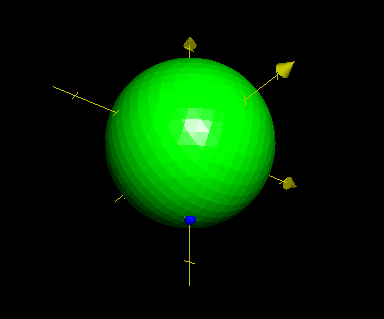
\includegraphics{quantum_state_0.png}
\caption{quantum\_state\_0.png}
\end{figure}

    The north pole represents the basis state

\begin{align}
|1\rangle = \begin{pmatrix} 0\\1 \end{pmatrix}
\end{align}

    \begin{figure}
\centering
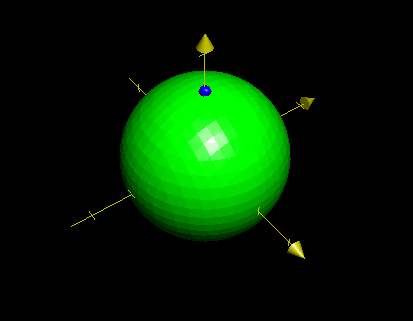
\includegraphics{quantum_state_1.png}
\caption{quantum\_state\_1.png}
\end{figure}

    We can also form linear combinations of the two basis states:

\begin{align}
\alpha |0\rangle + \beta |1 \rangle = \begin{pmatrix} \alpha \\ \beta \end{pmatrix}
\end{align}

The coefficients \(\alpha\) and \(\beta\), which always satify the
condition we derived \(|\alpha|^2+|\beta|^2 = 1\), the corresponding
point on the Bloch sphere will move to some other location.

    \hypertarget{common-basis-states}{%
\subsubsection{Common Basis States}\label{common-basis-states}}

    The \(x\)-axis, \(y\)-axis, and \(z\)-axis define three \textbf{bases}
in which to perform computation. The \(z\)-axis is the standard
computational basis. This is the ``spin-up/spin-down'' states and the
other basis states can be defined in terms of this basis. Really any of
the basis states can be defined in terms of the others, but generally
one starts with the \(z\)-axis basis \(|0\rangle\) and \(|1\rangle\).

    \hypertarget{spin-upspin-down-z-axis}{%
\paragraph{Spin-up/Spin-down (z-axis)}\label{spin-upspin-down-z-axis}}

\begin{align}
\text{spin-down}: \ |0\rangle &= \begin{pmatrix} 1\\0 \end{pmatrix} \\
\text{spin-up}: \ |1\rangle & = \begin{pmatrix} 0\\1 \end{pmatrix}
\end{align}

    \hypertarget{spin-rightspin-left-x-axis}{%
\paragraph{Spin-right/Spin-left
(x-axis)}\label{spin-rightspin-left-x-axis}}

\begin{align}
\text{spin-right}: \ |r\rangle &= \begin{pmatrix} 1/\sqrt{2} \\ 1/\sqrt{2} \end{pmatrix} = \frac{1}{\sqrt{2}} \left(|0\rangle + |1\rangle\right) \\
\text{spin-left}: \ |l\rangle & = \begin{pmatrix} 1/\sqrt{2} \\ -1/\sqrt{2} \end{pmatrix} = \frac{1}{\sqrt{2}} \left(|0\rangle - |1\rangle\right)
\end{align}

    \hypertarget{spin-spin---y-axis}{%
\paragraph{Spin +/Spin - (y-axis)}\label{spin-spin---y-axis}}

\begin{align}
\text{spin +}: \ |+\rangle &= \begin{pmatrix} 1/\sqrt{2} \\ i/\sqrt{2} \end{pmatrix} = \frac{1}{\sqrt{2}} \left(|0\rangle + i|1\rangle\right) \\
\text{spin -}: \ |-\rangle & = \begin{pmatrix} 1/\sqrt{2} \\ -i/\sqrt{2} \end{pmatrix} = \frac{1}{\sqrt{2}} \left(|0\rangle - i|1\rangle\right)
\end{align}

    \hypertarget{arbitrary-pure-state}{%
\paragraph{Arbitrary Pure State}\label{arbitrary-pure-state}}

An arbitrary pure state is represented as some linear combination:

\begin{align}
|\psi \rangle =
\begin{pmatrix}
\alpha \\ \beta
\end{pmatrix} = \alpha |0\rangle + \beta |1\rangle
\end{align}

    \begin{figure}
\centering
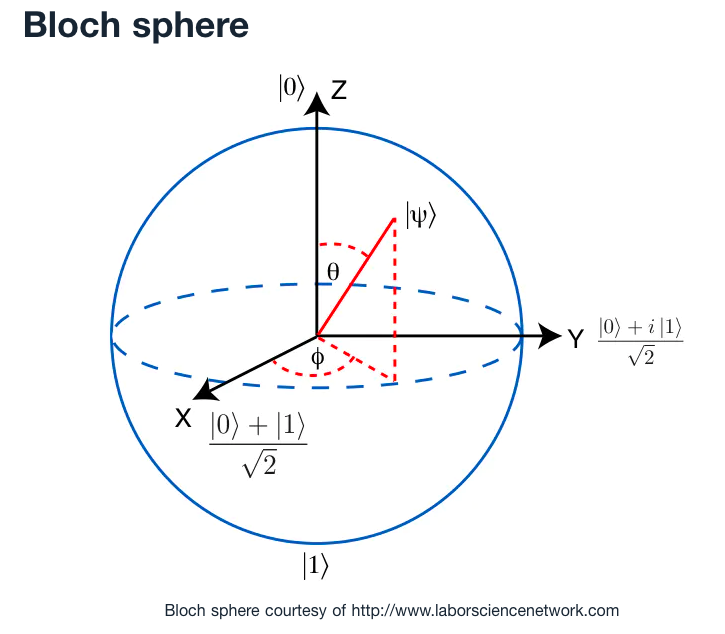
\includegraphics{Bloch_sphere.png}
\caption{Bloch\_sphere.png}
\end{figure}

    This image was taken from
\href{https://www.quantum-inspire.com/kbase/bloch-sphere/}{Quantum
Inspire}.

    We can define the six basis states in Python as follows:

    \begin{tcolorbox}[breakable, size=fbox, boxrule=1pt, pad at break*=1mm,colback=cellbackground, colframe=cellborder]
\prompt{In}{incolor}{27}{\hspace{4pt}}
\begin{Verbatim}[commandchars=\\\{\}]
\PY{n}{spin\PYZus{}down} \PY{o}{=} \PY{n}{np}\PY{o}{.}\PY{n}{matrix}\PY{p}{(}\PY{p}{[}\PY{p}{[}\PY{l+m+mi}{1}\PY{p}{]}\PY{p}{,} 
                       \PY{p}{[}\PY{l+m+mi}{0}\PY{p}{]}\PY{p}{]}\PY{p}{)}

\PY{n}{spin\PYZus{}up} \PY{o}{=} \PY{n}{np}\PY{o}{.}\PY{n}{matrix}\PY{p}{(}\PY{p}{[}\PY{p}{[}\PY{l+m+mi}{0}\PY{p}{]}\PY{p}{,}
                     \PY{p}{[}\PY{l+m+mi}{1}\PY{p}{]}\PY{p}{]}\PY{p}{)}

\PY{n}{spin\PYZus{}right} \PY{o}{=} \PY{p}{(}\PY{l+m+mi}{1}\PY{o}{/}\PY{n}{np}\PY{o}{.}\PY{n}{sqrt}\PY{p}{(}\PY{l+m+mi}{2}\PY{p}{)}\PY{p}{)}\PY{o}{*}\PY{p}{(}\PY{n}{spin\PYZus{}down} \PY{o}{+} \PY{n}{spin\PYZus{}up}\PY{p}{)}

\PY{n}{spin\PYZus{}left} \PY{o}{=} \PY{p}{(}\PY{l+m+mi}{1}\PY{o}{/}\PY{n}{np}\PY{o}{.}\PY{n}{sqrt}\PY{p}{(}\PY{l+m+mi}{2}\PY{p}{)}\PY{p}{)}\PY{o}{*}\PY{p}{(}\PY{n}{spin\PYZus{}down} \PY{o}{\PYZhy{}} \PY{n}{spin\PYZus{}up}\PY{p}{)}

\PY{n}{spin\PYZus{}plus} \PY{o}{=} \PY{p}{(}\PY{l+m+mi}{1}\PY{o}{/}\PY{n}{np}\PY{o}{.}\PY{n}{sqrt}\PY{p}{(}\PY{l+m+mi}{2}\PY{p}{)}\PY{p}{)}\PY{o}{*}\PY{p}{(}\PY{n}{spin\PYZus{}down} \PY{o}{+} \PY{l+m+mi}{1}\PY{n}{j}\PY{o}{*}\PY{n}{spin\PYZus{}up}\PY{p}{)}

\PY{n}{spin\PYZus{}minus} \PY{o}{=} \PY{p}{(}\PY{l+m+mi}{1}\PY{o}{/}\PY{n}{np}\PY{o}{.}\PY{n}{sqrt}\PY{p}{(}\PY{l+m+mi}{2}\PY{p}{)}\PY{p}{)}\PY{o}{*}\PY{p}{(}\PY{n}{spin\PYZus{}down} \PY{o}{\PYZhy{}} \PY{l+m+mi}{1}\PY{n}{j}\PY{o}{*}\PY{n}{spin\PYZus{}up}\PY{p}{)}

\PY{n+nb}{print}\PY{p}{(}\PY{l+s+s1}{\PYZsq{}}\PY{l+s+s1}{spin down:}\PY{l+s+s1}{\PYZsq{}}\PY{p}{,} \PY{n}{spin\PYZus{}down}\PY{p}{)}
\PY{n+nb}{print}\PY{p}{(}\PY{l+s+s1}{\PYZsq{}}\PY{l+s+s1}{spin up:}\PY{l+s+s1}{\PYZsq{}}\PY{p}{,} \PY{n}{spin\PYZus{}up}\PY{p}{)}
\PY{n+nb}{print}\PY{p}{(}\PY{l+s+s1}{\PYZsq{}}\PY{l+s+s1}{spin right:}\PY{l+s+s1}{\PYZsq{}}\PY{p}{,} \PY{n}{spin\PYZus{}right}\PY{p}{)}
\PY{n+nb}{print}\PY{p}{(}\PY{l+s+s1}{\PYZsq{}}\PY{l+s+s1}{spin left:}\PY{l+s+s1}{\PYZsq{}}\PY{p}{,} \PY{n}{spin\PYZus{}left}\PY{p}{)}
\PY{n+nb}{print}\PY{p}{(}\PY{l+s+s1}{\PYZsq{}}\PY{l+s+s1}{spin plus:}\PY{l+s+s1}{\PYZsq{}}\PY{p}{,} \PY{n}{spin\PYZus{}plus}\PY{p}{)}
\PY{n+nb}{print}\PY{p}{(}\PY{l+s+s1}{\PYZsq{}}\PY{l+s+s1}{spin minus:}\PY{l+s+s1}{\PYZsq{}}\PY{p}{,} \PY{n}{spin\PYZus{}minus}\PY{p}{)}
\end{Verbatim}
\end{tcolorbox}

    \begin{Verbatim}[commandchars=\\\{\}]
spin down: [[1]
 [0]]
spin up: [[0]
 [1]]
spin right: [[0.70710678]
 [0.70710678]]
spin left: [[ 0.70710678]
 [-0.70710678]]
spin plus: [[0.70710678+0.j        ]
 [0.        +0.70710678j]]
spin minus: [[0.70710678+0.j        ]
 [0.        -0.70710678j]]
\end{Verbatim}

    We can now compute inner products like \(\langle 0|0 \rangle\) and
\(\langle l | r \rangle\):

    \begin{tcolorbox}[breakable, size=fbox, boxrule=1pt, pad at break*=1mm,colback=cellbackground, colframe=cellborder]
\prompt{In}{incolor}{28}{\hspace{4pt}}
\begin{Verbatim}[commandchars=\\\{\}]
\PY{n}{np}\PY{o}{.}\PY{n}{dot}\PY{p}{(}\PY{n}{spin\PYZus{}down}\PY{o}{.}\PY{n}{H}\PY{p}{,} \PY{n}{spin\PYZus{}down}\PY{p}{)}
\end{Verbatim}
\end{tcolorbox}

            \begin{tcolorbox}[breakable, boxrule=.5pt, size=fbox, pad at break*=1mm, opacityfill=0]
\prompt{Out}{outcolor}{28}{\hspace{3.5pt}}
\begin{Verbatim}[commandchars=\\\{\}]
matrix([[1]])
\end{Verbatim}
\end{tcolorbox}
        
    \begin{tcolorbox}[breakable, size=fbox, boxrule=1pt, pad at break*=1mm,colback=cellbackground, colframe=cellborder]
\prompt{In}{incolor}{29}{\hspace{4pt}}
\begin{Verbatim}[commandchars=\\\{\}]
\PY{n}{np}\PY{o}{.}\PY{n}{dot}\PY{p}{(}\PY{n}{spin\PYZus{}left}\PY{o}{.}\PY{n}{H}\PY{p}{,} \PY{n}{spin\PYZus{}right}\PY{p}{)}
\end{Verbatim}
\end{tcolorbox}

            \begin{tcolorbox}[breakable, boxrule=.5pt, size=fbox, pad at break*=1mm, opacityfill=0]
\prompt{Out}{outcolor}{29}{\hspace{3.5pt}}
\begin{Verbatim}[commandchars=\\\{\}]
matrix([[0.]])
\end{Verbatim}
\end{tcolorbox}
        
    \hypertarget{exercises}{%
\subsubsection{Exercises}\label{exercises}}

    Use the above code defining the six basis states to compute:

    \begin{enumerate}
\def\labelenumi{\arabic{enumi}.}
\tightlist
\item
  \(\langle 0 | 1 \rangle\)
\item
  \(\langle 1 | 0 \rangle\)
\item
  \(\langle 1 | 1 \rangle\)
\item
  \(\langle r | l \rangle\)
\item
  \(\langle l | r \rangle\)
\item
  \(\langle r | r \rangle\)
\item
  \(\langle l | l \rangle\)
\item
  \(\langle + | - \rangle\)
\item
  \(\langle + | r \rangle\)
\item
  \(\langle - | l \rangle\)
\item
  \(\langle 0 | r \rangle\)
\item
  \(\langle l | 1 \rangle\)
\item
  \(\langle 0 | + \rangle\)
\item
  \(\langle - | - \rangle\)
\item
  \(\langle - | r \rangle\)
\end{enumerate}

    \hypertarget{tensor-products-of-vectors}{%
\subsection{Tensor Products of
Vectors}\label{tensor-products-of-vectors}}

    One of the most common tensor products we will encounter throughout the
following chapters of the book will be the tensor product of two qubits,
which are represented by \(2\)-dimensional vector which have length (or
``norm'') \(1\).

The general rule for the tensor product of two \(2\)-dimensional vectors
is as follows:

\begin{align}
\begin{pmatrix}
a_1 \\ a_2
\end{pmatrix} \otimes
\begin{pmatrix}
b_1 \\ b_2
\end{pmatrix} = 
\begin{pmatrix}
a_1 \begin{pmatrix}
b_1 \\ b_2
\end{pmatrix} \\ a_2 \begin{pmatrix}
b_1 \\ b_2
\end{pmatrix}
\end{pmatrix} = 
\begin{pmatrix}
a_1b_1 \\ a_1b_2 \\ a_2b_1 \\ a_2b_2
\end{pmatrix}
\end{align}

    Here is a numerical example:

    \begin{align}
\begin{pmatrix}
2 \\ 5
\end{pmatrix} \otimes 
\begin{pmatrix}
3 \\ 1
\end{pmatrix} = 
\begin{pmatrix}
2 \begin{pmatrix}
3 \\ 1
\end{pmatrix} \\ 5 \begin{pmatrix}
3 \\ 1
\end{pmatrix}
\end{pmatrix} = 
\begin{pmatrix}
2 \cdot 3 \\ 2 \cdot 1 \\ 5 \cdot 3 \\ 5 \cdot 1
\end{pmatrix} = 
\begin{pmatrix}
6 \\ 2 \\ 15 \\ 5
\end{pmatrix}
\end{align}

    For an example using Python we will use the ``np.kron()'' function,
which is the
\href{https://en.wikipedia.org/wiki/Kronecker_product}{Kronecker
product},

\begin{quote}
``In mathematics, the Kronecker product, sometimes denoted by ⊗, is an
operation on two matrices of arbitrary size resulting in a block matrix.
It is a generalization of the outer product (which is denoted by the
same symbol) from vectors to matrices, and gives the matrix of the
tensor product with respect to a standard choice of basis. The Kronecker
product should not be confused with the usual matrix multiplication,
which is an entirely different operation.''
\end{quote}

    \begin{tcolorbox}[breakable, size=fbox, boxrule=1pt, pad at break*=1mm,colback=cellbackground, colframe=cellborder]
\prompt{In}{incolor}{30}{\hspace{4pt}}
\begin{Verbatim}[commandchars=\\\{\}]
\PY{c+c1}{\PYZsh{} Define two ket\PYZhy{}vectors}

\PY{n}{A} \PY{o}{=} \PY{n}{np}\PY{o}{.}\PY{n}{array}\PY{p}{(}\PY{p}{[}\PY{p}{[}\PY{l+m+mi}{2}\PY{p}{]}\PY{p}{,} 
              \PY{p}{[}\PY{l+m+mi}{5}\PY{p}{]}\PY{p}{]}\PY{p}{)}

\PY{n}{B} \PY{o}{=} \PY{n}{np}\PY{o}{.}\PY{n}{array}\PY{p}{(}\PY{p}{[}\PY{p}{[}\PY{l+m+mi}{3}\PY{p}{]}\PY{p}{,}
              \PY{p}{[}\PY{l+m+mi}{1}\PY{p}{]}\PY{p}{]}\PY{p}{)}

\PY{c+c1}{\PYZsh{} Take the Kronecker (tensor) product of the two column vectors}
\PY{n}{np}\PY{o}{.}\PY{n}{kron}\PY{p}{(}\PY{n}{A}\PY{p}{,}\PY{n}{B}\PY{p}{)}
\end{Verbatim}
\end{tcolorbox}

            \begin{tcolorbox}[breakable, boxrule=.5pt, size=fbox, pad at break*=1mm, opacityfill=0]
\prompt{Out}{outcolor}{30}{\hspace{3.5pt}}
\begin{Verbatim}[commandchars=\\\{\}]
array([[ 6],
       [ 2],
       [15],
       [ 5]])
\end{Verbatim}
\end{tcolorbox}
        
    We can also define these two vectors as matrices which will allow us to
compute Hermitian conjugates. The Kronecker product function `np.kron()'
will work all the same:

    \begin{tcolorbox}[breakable, size=fbox, boxrule=1pt, pad at break*=1mm,colback=cellbackground, colframe=cellborder]
\prompt{In}{incolor}{31}{\hspace{4pt}}
\begin{Verbatim}[commandchars=\\\{\}]
\PY{c+c1}{\PYZsh{} Define the ket\PYZhy{}vectors as 2x1 column matrices:}
\PY{n}{ket\PYZus{}A} \PY{o}{=} \PY{n}{np}\PY{o}{.}\PY{n}{matrix}\PY{p}{(}\PY{p}{[}\PY{p}{[}\PY{l+m+mi}{2}\PY{p}{]}\PY{p}{,} 
                   \PY{p}{[}\PY{l+m+mi}{5}\PY{p}{]}\PY{p}{]}\PY{p}{)}

\PY{n}{ket\PYZus{}B} \PY{o}{=} \PY{n}{np}\PY{o}{.}\PY{n}{matrix}\PY{p}{(}\PY{p}{[}\PY{p}{[}\PY{l+m+mi}{3}\PY{p}{]}\PY{p}{,} 
                   \PY{p}{[}\PY{l+m+mi}{1}\PY{p}{]}\PY{p}{]}\PY{p}{)}

\PY{c+c1}{\PYZsh{} Compute their Kronecker product}
\PY{n}{np}\PY{o}{.}\PY{n}{kron}\PY{p}{(}\PY{n}{ket\PYZus{}A}\PY{p}{,} \PY{n}{ket\PYZus{}B}\PY{p}{)}
\end{Verbatim}
\end{tcolorbox}

            \begin{tcolorbox}[breakable, boxrule=.5pt, size=fbox, pad at break*=1mm, opacityfill=0]
\prompt{Out}{outcolor}{31}{\hspace{3.5pt}}
\begin{Verbatim}[commandchars=\\\{\}]
matrix([[ 6],
        [ 2],
        [15],
        [ 5]])
\end{Verbatim}
\end{tcolorbox}
        
    This can also be done with complex vectors:

    \begin{tcolorbox}[breakable, size=fbox, boxrule=1pt, pad at break*=1mm,colback=cellbackground, colframe=cellborder]
\prompt{In}{incolor}{32}{\hspace{4pt}}
\begin{Verbatim}[commandchars=\\\{\}]
\PY{c+c1}{\PYZsh{} Define the ket\PYZhy{}vectors as 2x1 column matrices:}
\PY{n}{ket\PYZus{}psi} \PY{o}{=} \PY{n}{np}\PY{o}{.}\PY{n}{matrix}\PY{p}{(}\PY{p}{[}\PY{p}{[}\PY{l+m+mi}{2}\PY{o}{\PYZhy{}}\PY{l+m+mi}{1}\PY{n}{j}\PY{p}{]}\PY{p}{,} 
                     \PY{p}{[}\PY{l+m+mi}{3}\PY{n}{j}\PY{p}{]}\PY{p}{]}\PY{p}{)}

\PY{n}{ket\PYZus{}phi} \PY{o}{=} \PY{n}{np}\PY{o}{.}\PY{n}{matrix}\PY{p}{(}\PY{p}{[}\PY{p}{[}\PY{o}{\PYZhy{}}\PY{l+m+mi}{3}\PY{p}{]}\PY{p}{,} 
                     \PY{p}{[}\PY{l+m+mi}{4}\PY{o}{\PYZhy{}}\PY{l+m+mi}{2}\PY{n}{j}\PY{p}{]}\PY{p}{]}\PY{p}{)}

\PY{c+c1}{\PYZsh{} Compute their Kronecker product}
\PY{n}{np}\PY{o}{.}\PY{n}{kron}\PY{p}{(}\PY{n}{ket\PYZus{}psi}\PY{p}{,} \PY{n}{ket\PYZus{}phi}\PY{p}{)}
\end{Verbatim}
\end{tcolorbox}

            \begin{tcolorbox}[breakable, boxrule=.5pt, size=fbox, pad at break*=1mm, opacityfill=0]
\prompt{Out}{outcolor}{32}{\hspace{3.5pt}}
\begin{Verbatim}[commandchars=\\\{\}]
matrix([[-6. +3.j],
        [ 6. -8.j],
        [-0. -9.j],
        [ 6.+12.j]])
\end{Verbatim}
\end{tcolorbox}
        
    Here is a more complicated example with two vectors of different
dimensions:

    \begin{align}
\begin{pmatrix}
a_1 \\ a_2
\end{pmatrix} \otimes 
\begin{pmatrix}
b_1 \\ b_2 \\ b_3
\end{pmatrix} = 
\begin{pmatrix}
a_1 \begin{pmatrix}
b_1 \\ b_2 \\ b_3
\end{pmatrix} \\
a_2 \begin{pmatrix}
b_1 \\ b_2 \\ b_3
\end{pmatrix}
\end{pmatrix} = 
\begin{pmatrix}
a_1b_1 \\ a_1b_2 \\ a_1b_3 \\ a_2b_1 \\ a_2b_2 \\ a_2b_3
\end{pmatrix}
\end{align}

    Here is a corresponding numerical example:

\begin{align}
\begin{pmatrix}
1 \\ 4
\end{pmatrix} \otimes 
\begin{pmatrix}
5 \\ 2 \\ 4
\end{pmatrix} = 
\begin{pmatrix}
1 \begin{pmatrix}
5 \\ 2 \\ 4
\end{pmatrix} \\
4 \begin{pmatrix}
5 \\ 2 \\ 4
\end{pmatrix}
\end{pmatrix} = 
\begin{pmatrix}
5 \\ 2 \\ 4 \\ 20 \\ 8 \\ 16
\end{pmatrix}
\end{align}

    Here is the code for computing this tensor product:

    \begin{tcolorbox}[breakable, size=fbox, boxrule=1pt, pad at break*=1mm,colback=cellbackground, colframe=cellborder]
\prompt{In}{incolor}{33}{\hspace{4pt}}
\begin{Verbatim}[commandchars=\\\{\}]
\PY{n}{ket\PYZus{}X} \PY{o}{=} \PY{n}{np}\PY{o}{.}\PY{n}{matrix}\PY{p}{(}\PY{p}{[}\PY{p}{[}\PY{l+m+mi}{1}\PY{p}{]}\PY{p}{,} 
                   \PY{p}{[}\PY{l+m+mi}{4}\PY{p}{]}\PY{p}{]}\PY{p}{)}

\PY{n}{ket\PYZus{}Y} \PY{o}{=} \PY{n}{np}\PY{o}{.}\PY{n}{matrix}\PY{p}{(}\PY{p}{[}\PY{p}{[}\PY{l+m+mi}{5}\PY{p}{]}\PY{p}{,} 
                   \PY{p}{[}\PY{l+m+mi}{2}\PY{p}{]}\PY{p}{,} 
                   \PY{p}{[}\PY{l+m+mi}{4}\PY{p}{]}\PY{p}{]}\PY{p}{)}

\PY{n}{np}\PY{o}{.}\PY{n}{kron}\PY{p}{(}\PY{n}{ket\PYZus{}X}\PY{p}{,} \PY{n}{ket\PYZus{}Y}\PY{p}{)}
\end{Verbatim}
\end{tcolorbox}

            \begin{tcolorbox}[breakable, boxrule=.5pt, size=fbox, pad at break*=1mm, opacityfill=0]
\prompt{Out}{outcolor}{33}{\hspace{3.5pt}}
\begin{Verbatim}[commandchars=\\\{\}]
matrix([[ 5],
        [ 2],
        [ 4],
        [20],
        [ 8],
        [16]])
\end{Verbatim}
\end{tcolorbox}
        
    \hypertarget{exercises}{%
\subsubsection{Exercises}\label{exercises}}

    \begin{enumerate}
\def\labelenumi{\arabic{enumi}.}
\tightlist
\item
  Using the following rule, \begin{align}
  \begin{pmatrix}
  a_1 \\ a_2 \\ a_3
  \end{pmatrix} \otimes
  \begin{pmatrix}
  b_1 \\ b_2
  \end{pmatrix} = 
  \begin{pmatrix}
  a_1 \begin{pmatrix}
  b_1 \\ b_2
  \end{pmatrix} \\ a_2\begin{pmatrix}
  b_1 \\ b_2
  \end{pmatrix} \\ a_3\begin{pmatrix}
  b_1 \\ b_2
  \end{pmatrix}
  \end{pmatrix} = 
  \begin{pmatrix}
  a_1b_1 \\ a_1b_2 \\ a_2b_1 \\ a_2b_2 \\ a_3b_1 \\ a_3b_2
  \end{pmatrix}
  \end{align}
\end{enumerate}

compute the following tensor/Kroneckar product by hand:

\begin{align}
\begin{pmatrix}
2 \\ 7 \\ 3
\end{pmatrix} \otimes
\begin{pmatrix}
5 \\ 9
\end{pmatrix}
\end{align}

    \begin{enumerate}
\def\labelenumi{\arabic{enumi}.}
\setcounter{enumi}{1}
\tightlist
\item
  Write Python code to compute the above computation using the
  `np.kron()' function. Remember to define two column (ket) vectors as
  matrices first.
\end{enumerate}

    \begin{enumerate}
\def\labelenumi{\arabic{enumi}.}
\setcounter{enumi}{2}
\tightlist
\item
  Derive a general rule for the following tensor product by performing
  the tensor product inside the parenthesis first:
\end{enumerate}

\begin{align}
\left( \begin{pmatrix}
a_1 \\ a_2
\end{pmatrix} \otimes 
\begin{pmatrix}
b_1 \\ b_2
\end{pmatrix}\right) \otimes 
\begin{pmatrix}
c_1 \\ c_2
\end{pmatrix}
\end{align}

    \begin{enumerate}
\def\labelenumi{\arabic{enumi}.}
\setcounter{enumi}{3}
\tightlist
\item
  Now derive a general rule for the following tensor product by
  performing the tensor product in the parenthesis first:
\end{enumerate}

\begin{align}
\begin{pmatrix}
a_1 \\ a_2
\end{pmatrix} \otimes 
\left( \begin{pmatrix}
b_1 \\ b_2
\end{pmatrix} \otimes 
\begin{pmatrix}
c_1 \\ c_2
\end{pmatrix}\right)
\end{align}

Convince yourself that your results from the previous two computations
are in fact equal.

    \begin{enumerate}
\def\labelenumi{\arabic{enumi}.}
\setcounter{enumi}{4}
\tightlist
\item
  Write Python code to compute \$\textbar{}0\rangle \otimes \textbar{}0
  \rangle \$.
\item
  Write Python code to compute \$\textbar{}0\rangle \otimes \textbar{}1
  \rangle \$.
\item
  Write Python code to compute \$\textbar{}1\rangle \otimes \textbar{}0
  \rangle \$.
\item
  Write Python code to compute \$\textbar{}1\rangle \otimes \textbar{}1
  \rangle \$.
\end{enumerate}

    \hypertarget{preparing-basis-states-in-pennylane}{%
\subsection{Preparing Basis States in
PennyLane}\label{preparing-basis-states-in-pennylane}}

    In PennyLane, and other quantum computing software, we often want to
prepare basis states. This is something we will return to again in the
future when we study specific cases of quantum circuits, but having some
basic introduction to state preparation now seems appropriate since the
are simply tensor products of the basis states \(|0\rangle\) and
\(|1\rangle\). In particular, we can prepare states like

\begin{align}
|00 \rangle &= |0\rangle \otimes |0\rangle = \begin{pmatrix} 1\\0 \end{pmatrix} \otimes \begin{pmatrix} 1\\0 \end{pmatrix} = \begin{pmatrix} 1\\0\\0\\0 \end{pmatrix} \\
|01 \rangle &= |0\rangle \otimes |1\rangle = \begin{pmatrix} 1\\0 \end{pmatrix} \otimes \begin{pmatrix} 0\\1 \end{pmatrix} = \begin{pmatrix} 0\\1\\0\\0 \end{pmatrix} \\
|10 \rangle &= |1\rangle \otimes |0\rangle = \begin{pmatrix} 0\\1 \end{pmatrix} \otimes \begin{pmatrix} 1\\0 \end{pmatrix} = \begin{pmatrix} 0\\0\\1\\0 \end{pmatrix} \\
|11 \rangle &= |1\rangle \otimes |1\rangle = \begin{pmatrix} 0\\1 \end{pmatrix} \otimes \begin{pmatrix} 0\\1 \end{pmatrix} = \begin{pmatrix} 0\\0\\0\\1 \end{pmatrix}
\end{align}

    \begin{tcolorbox}[breakable, size=fbox, boxrule=1pt, pad at break*=1mm,colback=cellbackground, colframe=cellborder]
\prompt{In}{incolor}{34}{\hspace{4pt}}
\begin{Verbatim}[commandchars=\\\{\}]
\PY{c+c1}{\PYZsh{} Define the basis states:}

\PY{n}{down\PYZus{}down} \PY{o}{=} \PY{n}{np}\PY{o}{.}\PY{n}{kron}\PY{p}{(}\PY{n}{spin\PYZus{}down}\PY{p}{,} \PY{n}{spin\PYZus{}down}\PY{p}{)}
\PY{n}{down\PYZus{}up} \PY{o}{=} \PY{n}{np}\PY{o}{.}\PY{n}{kron}\PY{p}{(}\PY{n}{spin\PYZus{}down}\PY{p}{,} \PY{n}{spin\PYZus{}up}\PY{p}{)}
\PY{n}{up\PYZus{}down} \PY{o}{=} \PY{n}{np}\PY{o}{.}\PY{n}{kron}\PY{p}{(}\PY{n}{spin\PYZus{}up}\PY{p}{,} \PY{n}{spin\PYZus{}down}\PY{p}{)}
\PY{n}{up\PYZus{}up} \PY{o}{=} \PY{n}{np}\PY{o}{.}\PY{n}{kron}\PY{p}{(}\PY{n}{spin\PYZus{}up}\PY{p}{,} \PY{n}{spin\PYZus{}up}\PY{p}{)}

\PY{c+c1}{\PYZsh{} Print the first state:}
\PY{n+nb}{print}\PY{p}{(}\PY{l+s+s1}{\PYZsq{}}\PY{l+s+s1}{|00\PYZgt{} =}\PY{l+s+s1}{\PYZsq{}}\PY{p}{)}
\PY{n+nb}{print}\PY{p}{(}\PY{n}{down\PYZus{}down}\PY{p}{)}
\end{Verbatim}
\end{tcolorbox}

    \begin{Verbatim}[commandchars=\\\{\}]
|00> =
[[1]
 [0]
 [0]
 [0]]
\end{Verbatim}

    \begin{tcolorbox}[breakable, size=fbox, boxrule=1pt, pad at break*=1mm,colback=cellbackground, colframe=cellborder]
\prompt{In}{incolor}{35}{\hspace{4pt}}
\begin{Verbatim}[commandchars=\\\{\}]
\PY{c+c1}{\PYZsh{} Print the second state:}
\PY{n+nb}{print}\PY{p}{(}\PY{l+s+s1}{\PYZsq{}}\PY{l+s+s1}{|01\PYZgt{} =}\PY{l+s+s1}{\PYZsq{}}\PY{p}{)}
\PY{n+nb}{print}\PY{p}{(}\PY{n}{down\PYZus{}up}\PY{p}{)}
\end{Verbatim}
\end{tcolorbox}

    \begin{Verbatim}[commandchars=\\\{\}]
|01> =
[[0]
 [1]
 [0]
 [0]]
\end{Verbatim}

    \begin{tcolorbox}[breakable, size=fbox, boxrule=1pt, pad at break*=1mm,colback=cellbackground, colframe=cellborder]
\prompt{In}{incolor}{36}{\hspace{4pt}}
\begin{Verbatim}[commandchars=\\\{\}]
\PY{c+c1}{\PYZsh{} Print the third state:}
\PY{n+nb}{print}\PY{p}{(}\PY{l+s+s1}{\PYZsq{}}\PY{l+s+s1}{|10\PYZgt{} =}\PY{l+s+s1}{\PYZsq{}}\PY{p}{)} 
\PY{n+nb}{print}\PY{p}{(}\PY{n}{up\PYZus{}down}\PY{p}{)}
\end{Verbatim}
\end{tcolorbox}

    \begin{Verbatim}[commandchars=\\\{\}]
|10> =
[[0]
 [0]
 [1]
 [0]]
\end{Verbatim}

    \begin{tcolorbox}[breakable, size=fbox, boxrule=1pt, pad at break*=1mm,colback=cellbackground, colframe=cellborder]
\prompt{In}{incolor}{37}{\hspace{4pt}}
\begin{Verbatim}[commandchars=\\\{\}]
\PY{c+c1}{\PYZsh{} Print the fourth state:}
\PY{n+nb}{print}\PY{p}{(}\PY{l+s+s1}{\PYZsq{}}\PY{l+s+s1}{|11\PYZgt{} =}\PY{l+s+s1}{\PYZsq{}}\PY{p}{)} 
\PY{n+nb}{print}\PY{p}{(}\PY{n}{up\PYZus{}up}\PY{p}{)}
\end{Verbatim}
\end{tcolorbox}

    \begin{Verbatim}[commandchars=\\\{\}]
|11> =
[[0]
 [0]
 [0]
 [1]]
\end{Verbatim}

    Taking this further, we can define states like:

\begin{align}
|000\rangle = |0\rangle \otimes |0\rangle \otimes |0\rangle = \begin{pmatrix} 1\\0\\0\\0\\0\\0\\0\\0 \end{pmatrix}
\end{align}

\begin{align}
|010\rangle = |0\rangle \otimes |1\rangle \otimes |0\rangle = \begin{pmatrix} 0\\0\\1\\0\\0\\0\\0\\0 \end{pmatrix}
\end{align}

    In PennyLane the following code prepares defines a device (quantum
computer or simulator) on which to run code. We will use the default
simulator for now since the code is very simple and running it on an
actual quantum computer is unnecessary:

    \begin{tcolorbox}[breakable, size=fbox, boxrule=1pt, pad at break*=1mm,colback=cellbackground, colframe=cellborder]
\prompt{In}{incolor}{38}{\hspace{4pt}}
\begin{Verbatim}[commandchars=\\\{\}]
\PY{n}{dev} \PY{o}{=} \PY{n}{qml}\PY{o}{.}\PY{n}{device}\PY{p}{(}\PY{l+s+s2}{\PYZdq{}}\PY{l+s+s2}{default.qubit}\PY{l+s+s2}{\PYZdq{}}\PY{p}{,} \PY{n}{wires}\PY{o}{=}\PY{l+m+mi}{2}\PY{p}{,} \PY{n}{shots}\PY{o}{=}\PY{l+m+mi}{1}\PY{p}{)}
\end{Verbatim}
\end{tcolorbox}

    Now we can define an array that corresponds to the basis state
\(|00\rangle\):

    \begin{tcolorbox}[breakable, size=fbox, boxrule=1pt, pad at break*=1mm,colback=cellbackground, colframe=cellborder]
\prompt{In}{incolor}{39}{\hspace{4pt}}
\begin{Verbatim}[commandchars=\\\{\}]
\PY{n}{dd} \PY{o}{=} \PY{n}{np}\PY{o}{.}\PY{n}{array}\PY{p}{(}\PY{p}{[}\PY{l+m+mi}{0}\PY{p}{,} \PY{l+m+mi}{0}\PY{p}{]}\PY{p}{)}
\end{Verbatim}
\end{tcolorbox}

    Now, we define a `qnode' in PennyLane that samples the qubits and gives
a \(+1\) for spin-down and a \(-1\) for spin up:

    \begin{tcolorbox}[breakable, size=fbox, boxrule=1pt, pad at break*=1mm,colback=cellbackground, colframe=cellborder]
\prompt{In}{incolor}{40}{\hspace{4pt}}
\begin{Verbatim}[commandchars=\\\{\}]
\PY{n+nd}{@qml}\PY{o}{.}\PY{n}{qnode}\PY{p}{(}\PY{n}{dev}\PY{p}{)}
\PY{k}{def} \PY{n+nf}{circuit}\PY{p}{(}\PY{p}{)}\PY{p}{:}
    \PY{n}{qml}\PY{o}{.}\PY{n}{BasisState}\PY{p}{(}\PY{n}{dd}\PY{p}{,} \PY{n}{wires}\PY{o}{=}\PY{p}{[}\PY{l+m+mi}{0}\PY{p}{,} \PY{l+m+mi}{1}\PY{p}{]}\PY{p}{)}
    \PY{k}{return} \PY{n}{qml}\PY{o}{.}\PY{n}{sample}\PY{p}{(}\PY{n}{qml}\PY{o}{.}\PY{n}{PauliZ}\PY{p}{(}\PY{l+m+mi}{0}\PY{p}{)}\PY{p}{)}\PY{p}{,} \PY{n}{qml}\PY{o}{.}\PY{n}{sample}\PY{p}{(}\PY{n}{qml}\PY{o}{.}\PY{n}{PauliZ}\PY{p}{(}\PY{l+m+mi}{1}\PY{p}{)}\PY{p}{)}

\PY{n+nb}{print}\PY{p}{(}\PY{n}{circuit}\PY{p}{(}\PY{p}{)}\PY{p}{)}
\end{Verbatim}
\end{tcolorbox}

    \begin{Verbatim}[commandchars=\\\{\}]
[[1]
 [1]]
\end{Verbatim}

    The vector above show a \(+1\) in the first and second entry meaning it
is measuring two spin-up states. Let's define a new state to prepare
corresponding to \(|01 \rangle\):

    \begin{tcolorbox}[breakable, size=fbox, boxrule=1pt, pad at break*=1mm,colback=cellbackground, colframe=cellborder]
\prompt{In}{incolor}{41}{\hspace{4pt}}
\begin{Verbatim}[commandchars=\\\{\}]
\PY{n}{du} \PY{o}{=} \PY{n}{np}\PY{o}{.}\PY{n}{array}\PY{p}{(}\PY{p}{[}\PY{l+m+mi}{0}\PY{p}{,}\PY{l+m+mi}{1}\PY{p}{]}\PY{p}{)}
\end{Verbatim}
\end{tcolorbox}

    Next, let's define a new `qnode' do sample corresponding to this
prepared state:

    \begin{tcolorbox}[breakable, size=fbox, boxrule=1pt, pad at break*=1mm,colback=cellbackground, colframe=cellborder]
\prompt{In}{incolor}{42}{\hspace{4pt}}
\begin{Verbatim}[commandchars=\\\{\}]
\PY{n+nd}{@qml}\PY{o}{.}\PY{n}{qnode}\PY{p}{(}\PY{n}{dev}\PY{p}{)}
\PY{k}{def} \PY{n+nf}{circuit}\PY{p}{(}\PY{p}{)}\PY{p}{:}
    \PY{n}{qml}\PY{o}{.}\PY{n}{BasisState}\PY{p}{(}\PY{n}{du}\PY{p}{,} \PY{n}{wires}\PY{o}{=}\PY{p}{[}\PY{l+m+mi}{0}\PY{p}{,} \PY{l+m+mi}{1}\PY{p}{]}\PY{p}{)}
    \PY{k}{return} \PY{n}{qml}\PY{o}{.}\PY{n}{sample}\PY{p}{(}\PY{n}{qml}\PY{o}{.}\PY{n}{PauliZ}\PY{p}{(}\PY{l+m+mi}{0}\PY{p}{)}\PY{p}{)}\PY{p}{,} \PY{n}{qml}\PY{o}{.}\PY{n}{sample}\PY{p}{(}\PY{n}{qml}\PY{o}{.}\PY{n}{PauliZ}\PY{p}{(}\PY{l+m+mi}{1}\PY{p}{)}\PY{p}{)}

\PY{n+nb}{print}\PY{p}{(}\PY{n}{circuit}\PY{p}{(}\PY{p}{)}\PY{p}{)}
\end{Verbatim}
\end{tcolorbox}

    \begin{Verbatim}[commandchars=\\\{\}]
[[ 1]
 [-1]]
\end{Verbatim}

    As we can see, we get a \(+1\) in the first component, corresponding to
the spin-down state, and we get a \(-1\) in the second component
corresponding to the spin-up state. We can also tell PennyLane to
perform multiple ``shots'' or samples:

    \begin{tcolorbox}[breakable, size=fbox, boxrule=1pt, pad at break*=1mm,colback=cellbackground, colframe=cellborder]
\prompt{In}{incolor}{43}{\hspace{4pt}}
\begin{Verbatim}[commandchars=\\\{\}]
\PY{n}{dev2} \PY{o}{=} \PY{n}{qml}\PY{o}{.}\PY{n}{device}\PY{p}{(}\PY{l+s+s2}{\PYZdq{}}\PY{l+s+s2}{default.qubit}\PY{l+s+s2}{\PYZdq{}}\PY{p}{,} \PY{n}{wires}\PY{o}{=}\PY{l+m+mi}{2}\PY{p}{,} \PY{n}{shots}\PY{o}{=}\PY{l+m+mi}{10}\PY{p}{)}
\end{Verbatim}
\end{tcolorbox}

    If we define a new array corresponting to the state \(|11\rangle\):

    \begin{tcolorbox}[breakable, size=fbox, boxrule=1pt, pad at break*=1mm,colback=cellbackground, colframe=cellborder]
\prompt{In}{incolor}{44}{\hspace{4pt}}
\begin{Verbatim}[commandchars=\\\{\}]
\PY{n}{uu} \PY{o}{=} \PY{n}{np}\PY{o}{.}\PY{n}{array}\PY{p}{(}\PY{p}{[}\PY{l+m+mi}{1}\PY{p}{,}\PY{l+m+mi}{1}\PY{p}{]}\PY{p}{)}
\end{Verbatim}
\end{tcolorbox}

    We can define a new `qnode' with the new device we just defined, and we
should expect an output vector of

\begin{align}
\begin{pmatrix}
-1\\-1
\end{pmatrix}
\end{align}

ten times, corresponding to the ten samples:

    \begin{tcolorbox}[breakable, size=fbox, boxrule=1pt, pad at break*=1mm,colback=cellbackground, colframe=cellborder]
\prompt{In}{incolor}{45}{\hspace{4pt}}
\begin{Verbatim}[commandchars=\\\{\}]
\PY{n+nd}{@qml}\PY{o}{.}\PY{n}{qnode}\PY{p}{(}\PY{n}{dev2}\PY{p}{)}
\PY{k}{def} \PY{n+nf}{circuit}\PY{p}{(}\PY{p}{)}\PY{p}{:}
    \PY{n}{qml}\PY{o}{.}\PY{n}{BasisState}\PY{p}{(}\PY{n}{uu}\PY{p}{,} \PY{n}{wires}\PY{o}{=}\PY{p}{[}\PY{l+m+mi}{0}\PY{p}{,} \PY{l+m+mi}{1}\PY{p}{]}\PY{p}{)}
    \PY{k}{return} \PY{n}{qml}\PY{o}{.}\PY{n}{sample}\PY{p}{(}\PY{n}{qml}\PY{o}{.}\PY{n}{PauliZ}\PY{p}{(}\PY{l+m+mi}{0}\PY{p}{)}\PY{p}{)}\PY{p}{,} \PY{n}{qml}\PY{o}{.}\PY{n}{sample}\PY{p}{(}\PY{n}{qml}\PY{o}{.}\PY{n}{PauliZ}\PY{p}{(}\PY{l+m+mi}{1}\PY{p}{)}\PY{p}{)}

\PY{n+nb}{print}\PY{p}{(}\PY{n}{circuit}\PY{p}{(}\PY{p}{)}\PY{p}{)}
\end{Verbatim}
\end{tcolorbox}

    \begin{Verbatim}[commandchars=\\\{\}]
[[-1 -1 -1 -1 -1 -1 -1 -1 -1 -1]
 [-1 -1 -1 -1 -1 -1 -1 -1 -1 -1]]
\end{Verbatim}

    We will return to this when we discuss measurements and expectation
values.

    \hypertarget{exercises}{%
\subsubsection{Exercises}\label{exercises}}

    \hypertarget{write-code-to-compute-the-following-basis-states}{%
\paragraph{Write code to compute the following basis
states:}\label{write-code-to-compute-the-following-basis-states}}

\begin{enumerate}
\def\labelenumi{\arabic{enumi}.}
\tightlist
\item
  \(|000 \rangle\)
\item
  \(|001 \rangle\)
\item
  \(|010 \rangle\)
\item
  \(|011 \rangle\)
\item
  \(|100 \rangle\)
\item
  \(|101 \rangle\)
\item
  \(|110 \rangle\)
\item
  \(|111 \rangle\)
\end{enumerate}

Now, compute these by hand to verify your code is correct. For example,
the first computation will be

\begin{align}
\begin{pmatrix} 1\\0 \end{pmatrix} \otimes
\begin{pmatrix} 1\\0 \end{pmatrix} \otimes
\begin{pmatrix} 0\\1 \end{pmatrix}
\end{align}

    \begin{enumerate}
\def\labelenumi{\arabic{enumi}.}
\setcounter{enumi}{8}
\tightlist
\item
  Define a defaul device with ``3 wires'' and ``5 shots''.
\item
  Define an array `uud' for the basis state \(|001\rangle\).
\item
  Now define a `qnode' that will print the samples: \textgreater{}
  qml.sample(qml.PauliZ(0)), qml.sample(qml.PauliZ(1)),
  qml.sample(qml.PauliZ(2))
\item
  Run your `qnode' and verify that you get the output vector
  \begin{align}
  \begin{pmatrix}
  1 \\ 1 \\ -1
  \end{pmatrix}
  \end{align}
\end{enumerate}

five times.

\begin{enumerate}
\def\labelenumi{\arabic{enumi}.}
\setcounter{enumi}{12}
\tightlist
\item
  Try doing this with the other basis states given in Exercises 1-8.
\end{enumerate}

    \hypertarget{matrices}{%
\subsection{Matrices}\label{matrices}}

    Matrices form the foundation for quantum gates, which are just
operations on qubits that move the points around the Bloch sphere.
Matrices are also called operators and (quantum) gates. They can operate
on a single qubit, or on many qubits simultaneously. The operators (or
matrices or gates) we will be using most are known as \emph{unitary
operators} or \emph{unitary matrices}. In this section we will discuss
basic matrix algebra and define unitary matrices.

    We have already seen two ways or realizing matrices in Python. Suppose
we have the following \(2 \times 2\) matrix

\begin{align}
M = \begin{pmatrix}
2-i & -3 \\
-5i & 2
\end{pmatrix}
\end{align}

We can define this matrix as an array, or as a matrix in Python:

    \begin{tcolorbox}[breakable, size=fbox, boxrule=1pt, pad at break*=1mm,colback=cellbackground, colframe=cellborder]
\prompt{In}{incolor}{46}{\hspace{4pt}}
\begin{Verbatim}[commandchars=\\\{\}]
\PY{n}{M} \PY{o}{=} \PY{n}{np}\PY{o}{.}\PY{n}{array}\PY{p}{(}\PY{p}{[}\PY{p}{[}\PY{l+m+mi}{2}\PY{o}{\PYZhy{}}\PY{l+m+mi}{1}\PY{n}{j}\PY{p}{,} \PY{o}{\PYZhy{}}\PY{l+m+mi}{3}\PY{p}{]}\PY{p}{,}
              \PY{p}{[}\PY{o}{\PYZhy{}}\PY{l+m+mi}{5}\PY{n}{j}\PY{p}{,} \PY{l+m+mi}{2}\PY{p}{]}\PY{p}{]}\PY{p}{)}

\PY{n+nb}{print}\PY{p}{(}\PY{n}{M}\PY{p}{)}
\end{Verbatim}
\end{tcolorbox}

    \begin{Verbatim}[commandchars=\\\{\}]
[[ 2.-1.j -3.+0.j]
 [-0.-5.j  2.+0.j]]
\end{Verbatim}

    \begin{tcolorbox}[breakable, size=fbox, boxrule=1pt, pad at break*=1mm,colback=cellbackground, colframe=cellborder]
\prompt{In}{incolor}{47}{\hspace{4pt}}
\begin{Verbatim}[commandchars=\\\{\}]
\PY{n}{M} \PY{o}{=} \PY{n}{np}\PY{o}{.}\PY{n}{matrix}\PY{p}{(}\PY{p}{[}\PY{p}{[}\PY{l+m+mi}{2}\PY{o}{\PYZhy{}}\PY{l+m+mi}{1}\PY{n}{j}\PY{p}{,} \PY{o}{\PYZhy{}}\PY{l+m+mi}{3}\PY{p}{]}\PY{p}{,}
               \PY{p}{[}\PY{o}{\PYZhy{}}\PY{l+m+mi}{5}\PY{n}{j}\PY{p}{,} \PY{l+m+mi}{2}\PY{p}{]}\PY{p}{]}\PY{p}{)}

\PY{n+nb}{print}\PY{p}{(}\PY{n}{M}\PY{p}{)}
\end{Verbatim}
\end{tcolorbox}

    \begin{Verbatim}[commandchars=\\\{\}]
[[ 2.-1.j -3.+0.j]
 [-0.-5.j  2.+0.j]]
\end{Verbatim}

    We will use the second version, the matrix version, so that we can again
take Hermitian conjugates of the matrices, which is again given by the
conjugate transpose:

    \begin{tcolorbox}[breakable, size=fbox, boxrule=1pt, pad at break*=1mm,colback=cellbackground, colframe=cellborder]
\prompt{In}{incolor}{48}{\hspace{4pt}}
\begin{Verbatim}[commandchars=\\\{\}]
\PY{n+nb}{print}\PY{p}{(}\PY{n}{M}\PY{o}{.}\PY{n}{H}\PY{p}{)}
\end{Verbatim}
\end{tcolorbox}

    \begin{Verbatim}[commandchars=\\\{\}]
[[ 2.+1.j -0.+5.j]
 [-3.-0.j  2.-0.j]]
\end{Verbatim}

    This transposes the matrix and conjugates all of its entries. We can
also multiply matrices so long as the dimensions match appropriately. In
particular, to multiply two matrices \(A\) and \(B\), the matrix must be
an \(n \times p\) matrix and the matrix \(B\) must be a \(p \times m\)
matrix. The result is an \(n \times m\) matrix. For example:

    \begin{tcolorbox}[breakable, size=fbox, boxrule=1pt, pad at break*=1mm,colback=cellbackground, colframe=cellborder]
\prompt{In}{incolor}{49}{\hspace{4pt}}
\begin{Verbatim}[commandchars=\\\{\}]
\PY{c+c1}{\PYZsh{} Define a 3x2 matrix:}
\PY{n}{A} \PY{o}{=} \PY{n}{np}\PY{o}{.}\PY{n}{matrix}\PY{p}{(}\PY{p}{[}\PY{p}{[}\PY{l+m+mi}{2}\PY{n}{j}\PY{p}{,} \PY{o}{\PYZhy{}}\PY{l+m+mi}{5}\PY{p}{]}\PY{p}{,}
               \PY{p}{[}\PY{l+m+mi}{3}\PY{o}{\PYZhy{}}\PY{l+m+mi}{5}\PY{n}{j}\PY{p}{,} \PY{l+m+mi}{1}\PY{p}{]}\PY{p}{,} 
               \PY{p}{[}\PY{l+m+mi}{5}\PY{p}{,} \PY{l+m+mi}{4}\PY{n}{j}\PY{p}{]}\PY{p}{]}\PY{p}{)}

\PY{c+c1}{\PYZsh{} Define a 2x4 matrix:}
\PY{n}{B} \PY{o}{=} \PY{n}{np}\PY{o}{.}\PY{n}{matrix}\PY{p}{(}\PY{p}{[}\PY{p}{[}\PY{l+m+mi}{1}\PY{p}{,} \PY{o}{\PYZhy{}}\PY{l+m+mi}{3}\PY{n}{j}\PY{p}{,} \PY{l+m+mi}{5}\PY{p}{,} \PY{l+m+mi}{2}\PY{p}{]}\PY{p}{,} 
               \PY{p}{[}\PY{l+m+mi}{1}\PY{o}{\PYZhy{}}\PY{l+m+mi}{1}\PY{n}{j}\PY{p}{,} \PY{l+m+mi}{1}\PY{p}{,} \PY{l+m+mi}{3}\PY{p}{,} \PY{l+m+mi}{7}\PY{n}{j}\PY{p}{]}\PY{p}{]}\PY{p}{)}

\PY{c+c1}{\PYZsh{}Taking the product of a (3x2) and (2x4) matrix will give a 3x4 matrix:}
\PY{n}{np}\PY{o}{.}\PY{n}{dot}\PY{p}{(}\PY{n}{A}\PY{p}{,} \PY{n}{B}\PY{p}{)}
\end{Verbatim}
\end{tcolorbox}

            \begin{tcolorbox}[breakable, boxrule=.5pt, size=fbox, pad at break*=1mm, opacityfill=0]
\prompt{Out}{outcolor}{49}{\hspace{3.5pt}}
\begin{Verbatim}[commandchars=\\\{\}]
matrix([[ -5. +7.j,   1. +0.j, -15.+10.j,   0.-31.j],
        [  4. -6.j, -14. -9.j,  18.-25.j,   6. -3.j],
        [  9. +4.j,   0.-11.j,  25.+12.j, -18. +0.j]])
\end{Verbatim}
\end{tcolorbox}
        
    If we are using the matrix definition instead of the array definition we
can also multiply the two matrices as follows:

    \begin{tcolorbox}[breakable, size=fbox, boxrule=1pt, pad at break*=1mm,colback=cellbackground, colframe=cellborder]
\prompt{In}{incolor}{50}{\hspace{4pt}}
\begin{Verbatim}[commandchars=\\\{\}]
\PY{n}{A}\PY{o}{*}\PY{n}{B}
\end{Verbatim}
\end{tcolorbox}

            \begin{tcolorbox}[breakable, boxrule=.5pt, size=fbox, pad at break*=1mm, opacityfill=0]
\prompt{Out}{outcolor}{50}{\hspace{3.5pt}}
\begin{Verbatim}[commandchars=\\\{\}]
matrix([[ -5. +7.j,   1. +0.j, -15.+10.j,   0.-31.j],
        [  4. -6.j, -14. -9.j,  18.-25.j,   6. -3.j],
        [  9. +4.j,   0.-11.j,  25.+12.j, -18. +0.j]])
\end{Verbatim}
\end{tcolorbox}
        
    If we define the two matrices as arrays, this will not work and will
return an error.

    \hypertarget{exercises}{%
\subsubsection{Exercises}\label{exercises}}

    \hypertarget{define-the-following-four-matrices}{%
\paragraph{Define the following four
matrices}\label{define-the-following-four-matrices}}

\begin{align}
I = \begin{pmatrix} 1&0 \\ 0&1 \end{pmatrix}, \quad
X = \begin{pmatrix} 0&1 \\ 1&0 \end{pmatrix}, \quad
Y = \begin{pmatrix} 0&i \\ -i&0 \end{pmatrix}, \quad
Z = \begin{pmatrix} 1&0 \\ 0&-1 \end{pmatrix}, \quad
H = \frac{1}{\sqrt{2}} \begin{pmatrix} 1&1 \\ 1&-1 \end{pmatrix}
\end{align}

    \hypertarget{write-python-code-to-compute-the-following-matrix-multiplications}{%
\paragraph{Write Python code to compute the following matrix
multiplications:}\label{write-python-code-to-compute-the-following-matrix-multiplications}}

\begin{enumerate}
\def\labelenumi{\arabic{enumi}.}
\tightlist
\item
  \(XY\)
\item
  \(YX\)
\item
  \(YZ\)
\item
  \(ZY\)
\item
  \(HX\)
\item
  \(YH\)
\item
  \(XYZ\)
\item
  \(YZX\)
\item
  \(ZXY\)
\item
  \(XHY\)
\end{enumerate}

    \hypertarget{tensor-products-of-matrices}{%
\subsection{Tensor Products of
Matrices}\label{tensor-products-of-matrices}}

    In this section we will discuss how to take tensor products of matrices
in order to later build quantum gates that operate on many qubits at
once. Understanding the basics of tensor products of matrices is
fundamental to understanding quantum logic gates and quantum circuits.
For the tensor product of two \(2 \times 2\) matrices, the general rule
is as follows:

    \begin{align}
\begin{pmatrix}
a & b \\
c & d
\end{pmatrix} \otimes 
\begin{pmatrix}
x & y \\
z & w
\end{pmatrix} = 
\begin{pmatrix}
a \begin{pmatrix}
x & y \\
z & w
\end{pmatrix} & b \begin{pmatrix}
x & y \\
z & w
\end{pmatrix} \\
c \begin{pmatrix}
x & y \\
z & w
\end{pmatrix} & d \begin{pmatrix}
x & y \\
z & w
\end{pmatrix}
\end{pmatrix} = 
\begin{pmatrix}
ax & ay & bx & by \\
az & aw & bz & bw \\
cx & cy & dx & dy \\
cz & cw & dz & dw
\end{pmatrix}
\end{align}

    Here is a basic numerical example:

\begin{align}
\begin{pmatrix}
2 & 3 \\
6 & 1
\end{pmatrix} \otimes
\begin{pmatrix}
7 & 10 \\
9 & 4
\end{pmatrix} = 
\begin{pmatrix}
2 \begin{pmatrix}
7 & 10 \\
9 & 4
\end{pmatrix}& 3\begin{pmatrix}
7 & 10 \\
9 & 4
\end{pmatrix} \\
6\begin{pmatrix}
7 & 10 \\
9 & 4
\end{pmatrix} & 1\begin{pmatrix}
7 & 10 \\
9 & 4
\end{pmatrix}
\end{pmatrix} = 
\begin{pmatrix}
14 & 20 & 21 & 30 \\
18 & 8 & 27 & 12 \\
42 & 60 & 7 & 10 \\
54 & 24 & 9 & 4
\end{pmatrix}
\end{align}

    We can again use the `np.kron()' function to perform this computation in
Python:

    \begin{tcolorbox}[breakable, size=fbox, boxrule=1pt, pad at break*=1mm,colback=cellbackground, colframe=cellborder]
\prompt{In}{incolor}{51}{\hspace{4pt}}
\begin{Verbatim}[commandchars=\\\{\}]
\PY{n}{A} \PY{o}{=} \PY{n}{np}\PY{o}{.}\PY{n}{matrix}\PY{p}{(}\PY{p}{[}\PY{p}{[}\PY{l+m+mi}{2}\PY{p}{,} \PY{l+m+mi}{3}\PY{p}{]}\PY{p}{,}
               \PY{p}{[}\PY{l+m+mi}{6}\PY{p}{,} \PY{l+m+mi}{1}\PY{p}{]}\PY{p}{]}\PY{p}{)}

\PY{n}{B} \PY{o}{=} \PY{n}{np}\PY{o}{.}\PY{n}{matrix}\PY{p}{(}\PY{p}{[}\PY{p}{[}\PY{l+m+mi}{7}\PY{p}{,} \PY{l+m+mi}{10}\PY{p}{]}\PY{p}{,} 
               \PY{p}{[}\PY{l+m+mi}{9}\PY{p}{,} \PY{l+m+mi}{4}\PY{p}{]}\PY{p}{]}\PY{p}{)}

\PY{n}{np}\PY{o}{.}\PY{n}{kron}\PY{p}{(}\PY{n}{A}\PY{p}{,}\PY{n}{B}\PY{p}{)}
\end{Verbatim}
\end{tcolorbox}

            \begin{tcolorbox}[breakable, boxrule=.5pt, size=fbox, pad at break*=1mm, opacityfill=0]
\prompt{Out}{outcolor}{51}{\hspace{3.5pt}}
\begin{Verbatim}[commandchars=\\\{\}]
matrix([[14, 20, 21, 30],
        [18,  8, 27, 12],
        [42, 60,  7, 10],
        [54, 24,  9,  4]])
\end{Verbatim}
\end{tcolorbox}
        
    In quantum computing, if we have basis states such as

\begin{align}
|010\rangle &= |0\rangle \otimes |1\rangle \otimes |0\rangle \\
&= \begin{pmatrix}
1\\0
\end{pmatrix} \otimes 
\begin{pmatrix}
0\\1
\end{pmatrix} \otimes 
\begin{pmatrix}
1\\0
\end{pmatrix} \\
&= \begin{pmatrix}
0\\0\\1\\0\\0\\0\\0\\0
\end{pmatrix}
\end{align}

we can operate on them using tensor product of operators. In particular,
to operate on a three qubit basis state such at this, we need the tensor
product of three \(2 \times 2\) matrix. For example, with the following
four operators:

\begin{align}
I = \begin{pmatrix} 1&0 \\ 0&1 \end{pmatrix}, \quad
X = \begin{pmatrix} 0&1 \\ 1&0 \end{pmatrix}, \quad
Y = \begin{pmatrix} 0&i \\ -i&0 \end{pmatrix}, \quad
Z = \begin{pmatrix} 1&0 \\ 0&-1 \end{pmatrix}, \quad
H = \frac{1}{\sqrt{2}} \begin{pmatrix} 1&1 \\ 1&-1 \end{pmatrix}
\end{align}

We can form tensor product such as \(H \otimes X \otimes I\) and
\(Z \otimes Z \otimes H\), and any other three matrix combination you
might dream up. Let's define a basis state \(|01\rangle\) and compute a
few operators that will operate on this basis state:

    \begin{tcolorbox}[breakable, size=fbox, boxrule=1pt, pad at break*=1mm,colback=cellbackground, colframe=cellborder]
\prompt{In}{incolor}{52}{\hspace{4pt}}
\begin{Verbatim}[commandchars=\\\{\}]
\PY{c+c1}{\PYZsh{}Define the basis state |01\PYZgt{}}
\PY{n}{du} \PY{o}{=} \PY{n}{np}\PY{o}{.}\PY{n}{kron}\PY{p}{(}\PY{n}{spin\PYZus{}down}\PY{p}{,} \PY{n}{spin\PYZus{}up}\PY{p}{)}
\PY{n+nb}{print}\PY{p}{(}\PY{n}{du}\PY{p}{)}
\end{Verbatim}
\end{tcolorbox}

    \begin{Verbatim}[commandchars=\\\{\}]
[[0]
 [1]
 [0]
 [0]]
\end{Verbatim}

    \begin{tcolorbox}[breakable, size=fbox, boxrule=1pt, pad at break*=1mm,colback=cellbackground, colframe=cellborder]
\prompt{In}{incolor}{53}{\hspace{4pt}}
\begin{Verbatim}[commandchars=\\\{\}]
\PY{c+c1}{\PYZsh{} Define the matrices X, Y, Z, and H}
\PY{n}{X} \PY{o}{=} \PY{n}{np}\PY{o}{.}\PY{n}{matrix}\PY{p}{(}\PY{p}{[}\PY{p}{[}\PY{l+m+mi}{0}\PY{p}{,} \PY{l+m+mi}{1}\PY{p}{]}\PY{p}{,}
               \PY{p}{[}\PY{l+m+mi}{1}\PY{p}{,} \PY{l+m+mi}{0}\PY{p}{]}\PY{p}{]}\PY{p}{)}

\PY{n}{Y} \PY{o}{=} \PY{n}{np}\PY{o}{.}\PY{n}{matrix}\PY{p}{(}\PY{p}{[}\PY{p}{[}\PY{l+m+mi}{0}\PY{p}{,} \PY{o}{\PYZhy{}}\PY{l+m+mi}{1}\PY{n}{j}\PY{p}{]}\PY{p}{,} 
               \PY{p}{[}\PY{l+m+mi}{1}\PY{n}{j}\PY{p}{,} \PY{l+m+mi}{0}\PY{p}{]}\PY{p}{]}\PY{p}{)}

\PY{n}{Z} \PY{o}{=} \PY{n}{np}\PY{o}{.}\PY{n}{matrix}\PY{p}{(}\PY{p}{[}\PY{p}{[}\PY{l+m+mi}{1}\PY{p}{,} \PY{l+m+mi}{0}\PY{p}{]}\PY{p}{,}
               \PY{p}{[}\PY{l+m+mi}{0}\PY{p}{,} \PY{o}{\PYZhy{}}\PY{l+m+mi}{1}\PY{p}{]}\PY{p}{]}\PY{p}{)}

\PY{n}{H} \PY{o}{=} \PY{p}{(}\PY{l+m+mi}{1}\PY{o}{/}\PY{n}{np}\PY{o}{.}\PY{n}{sqrt}\PY{p}{(}\PY{l+m+mi}{2}\PY{p}{)}\PY{p}{)}\PY{o}{*}\PY{n}{np}\PY{o}{.}\PY{n}{matrix}\PY{p}{(}\PY{p}{[}\PY{p}{[}\PY{l+m+mi}{1}\PY{p}{,} \PY{l+m+mi}{1}\PY{p}{]}\PY{p}{,} 
                          \PY{p}{[}\PY{l+m+mi}{1}\PY{p}{,} \PY{o}{\PYZhy{}}\PY{l+m+mi}{1}\PY{p}{]}\PY{p}{]}\PY{p}{)}
\end{Verbatim}
\end{tcolorbox}

    Now let's comute the following four tensor products:

\begin{align}
X \otimes Y, \quad X \otimes Z, \quad H \otimes H
\end{align}

    \begin{tcolorbox}[breakable, size=fbox, boxrule=1pt, pad at break*=1mm,colback=cellbackground, colframe=cellborder]
\prompt{In}{incolor}{54}{\hspace{4pt}}
\begin{Verbatim}[commandchars=\\\{\}]
\PY{n+nb}{print}\PY{p}{(}\PY{n}{np}\PY{o}{.}\PY{n}{kron}\PY{p}{(}\PY{n}{X}\PY{p}{,} \PY{n}{Y}\PY{p}{)}\PY{p}{)}
\end{Verbatim}
\end{tcolorbox}

    \begin{Verbatim}[commandchars=\\\{\}]
[[0.+0.j 0.-0.j 0.+0.j 0.-1.j]
 [0.+0.j 0.+0.j 0.+1.j 0.+0.j]
 [0.+0.j 0.-1.j 0.+0.j 0.-0.j]
 [0.+1.j 0.+0.j 0.+0.j 0.+0.j]]
\end{Verbatim}

    \begin{tcolorbox}[breakable, size=fbox, boxrule=1pt, pad at break*=1mm,colback=cellbackground, colframe=cellborder]
\prompt{In}{incolor}{55}{\hspace{4pt}}
\begin{Verbatim}[commandchars=\\\{\}]
\PY{n+nb}{print}\PY{p}{(}\PY{n}{np}\PY{o}{.}\PY{n}{kron}\PY{p}{(}\PY{n}{X}\PY{p}{,} \PY{n}{Z}\PY{p}{)}\PY{p}{)}
\end{Verbatim}
\end{tcolorbox}

    \begin{Verbatim}[commandchars=\\\{\}]
[[ 0  0  1  0]
 [ 0  0  0 -1]
 [ 1  0  0  0]
 [ 0 -1  0  0]]
\end{Verbatim}

    \begin{tcolorbox}[breakable, size=fbox, boxrule=1pt, pad at break*=1mm,colback=cellbackground, colframe=cellborder]
\prompt{In}{incolor}{56}{\hspace{4pt}}
\begin{Verbatim}[commandchars=\\\{\}]
\PY{n+nb}{print}\PY{p}{(}\PY{n}{np}\PY{o}{.}\PY{n}{kron}\PY{p}{(}\PY{n}{H}\PY{p}{,} \PY{n}{H}\PY{p}{)}\PY{p}{)}
\end{Verbatim}
\end{tcolorbox}

    \begin{Verbatim}[commandchars=\\\{\}]
[[ 0.5  0.5  0.5  0.5]
 [ 0.5 -0.5  0.5 -0.5]
 [ 0.5  0.5 -0.5 -0.5]
 [ 0.5 -0.5 -0.5  0.5]]
\end{Verbatim}

    Now, we can compute the action of these matrices on \(|01\rangle\) as:

\begin{align}
(X \otimes Y)(|01\rangle) = (X \otimes Y)(|0\rangle \otimes |1\rangle) = X|0\rangle \otimes Y|1\rangle 
\end{align}

\begin{align}
(X \otimes Z)(|01\rangle) = (X \otimes Z)(|0\rangle \otimes |1\rangle) = X|0\rangle \otimes Z|1\rangle 
\end{align}

\begin{align}
(H \otimes H)(|01\rangle) = (H \otimes H)(|0\rangle \otimes |1\rangle) = H|0\rangle \otimes H|1\rangle 
\end{align}

    \begin{tcolorbox}[breakable, size=fbox, boxrule=1pt, pad at break*=1mm,colback=cellbackground, colframe=cellborder]
\prompt{In}{incolor}{57}{\hspace{4pt}}
\begin{Verbatim}[commandchars=\\\{\}]
\PY{n}{XY} \PY{o}{=} \PY{n}{np}\PY{o}{.}\PY{n}{kron}\PY{p}{(}\PY{n}{X}\PY{p}{,} \PY{n}{Y}\PY{p}{)}
\PY{n}{XZ} \PY{o}{=} \PY{n}{np}\PY{o}{.}\PY{n}{kron}\PY{p}{(}\PY{n}{X}\PY{p}{,} \PY{n}{Z}\PY{p}{)}
\PY{n}{HH} \PY{o}{=} \PY{n}{np}\PY{o}{.}\PY{n}{kron}\PY{p}{(}\PY{n}{H}\PY{p}{,} \PY{n}{H}\PY{p}{)}
\end{Verbatim}
\end{tcolorbox}

    \begin{tcolorbox}[breakable, size=fbox, boxrule=1pt, pad at break*=1mm,colback=cellbackground, colframe=cellborder]
\prompt{In}{incolor}{58}{\hspace{4pt}}
\begin{Verbatim}[commandchars=\\\{\}]
\PY{n+nb}{print}\PY{p}{(}\PY{n}{XY} \PY{o}{*} \PY{n}{du}\PY{p}{)}
\end{Verbatim}
\end{tcolorbox}

    \begin{Verbatim}[commandchars=\\\{\}]
[[0.+0.j]
 [0.+0.j]
 [0.-1.j]
 [0.+0.j]]
\end{Verbatim}

    \begin{tcolorbox}[breakable, size=fbox, boxrule=1pt, pad at break*=1mm,colback=cellbackground, colframe=cellborder]
\prompt{In}{incolor}{59}{\hspace{4pt}}
\begin{Verbatim}[commandchars=\\\{\}]
\PY{n+nb}{print}\PY{p}{(}\PY{n}{XZ} \PY{o}{*} \PY{n}{du}\PY{p}{)}
\end{Verbatim}
\end{tcolorbox}

    \begin{Verbatim}[commandchars=\\\{\}]
[[ 0]
 [ 0]
 [ 0]
 [-1]]
\end{Verbatim}

    \begin{tcolorbox}[breakable, size=fbox, boxrule=1pt, pad at break*=1mm,colback=cellbackground, colframe=cellborder]
\prompt{In}{incolor}{60}{\hspace{4pt}}
\begin{Verbatim}[commandchars=\\\{\}]
\PY{n+nb}{print}\PY{p}{(}\PY{n}{HH} \PY{o}{*} \PY{n}{du}\PY{p}{)}
\end{Verbatim}
\end{tcolorbox}

    \begin{Verbatim}[commandchars=\\\{\}]
[[ 0.5]
 [-0.5]
 [ 0.5]
 [-0.5]]
\end{Verbatim}

    \hypertarget{exercises}{%
\subsubsection{Exercises}\label{exercises}}

    \begin{enumerate}
\def\labelenumi{\arabic{enumi}.}
\tightlist
\item
  Compute the following tensor product by hand:
\end{enumerate}

\begin{align}
\begin{pmatrix}
11 & 2 \\
3 & 5
\end{pmatrix} \otimes
\begin{pmatrix}
7 & 8 \\ 
0 & 1
\end{pmatrix}
\end{align}

    \hypertarget{compute-the-following-tensor-products-by-hand}{%
\paragraph{Compute the following tensor products by
hand:}\label{compute-the-following-tensor-products-by-hand}}

\begin{enumerate}
\def\labelenumi{\arabic{enumi}.}
\setcounter{enumi}{1}
\tightlist
\item
  \(X \otimes X\)
\item
  \(Z \otimes Y\)
\item
  \(H \otimes X\)
\end{enumerate}

    \hypertarget{write-python-code-to-compute-the-tensor-products}{%
\paragraph{Write Python code to compute the tensor
products:}\label{write-python-code-to-compute-the-tensor-products}}

\begin{enumerate}
\def\labelenumi{\arabic{enumi}.}
\setcounter{enumi}{4}
\tightlist
\item
  \(X \otimes X\)
\item
  \(Z \otimes Y\)
\item
  \(H \otimes X\)
\item
  \(H \otimes H\)
\end{enumerate}

    \begin{enumerate}
\def\labelenumi{\arabic{enumi}.}
\setcounter{enumi}{8}
\tightlist
\item
  Write Python code to verify that
  \((H \otimes H) \otimes H = H \otimes (H \otimes H)\).
\end{enumerate}

    \hypertarget{use-the-following-code-defining-the-basis-state-010-and-the-relevant-tensor-products-to-compute-the-following}{%
\paragraph{\texorpdfstring{Use the following code defining the basis
state \$\textbar{}010 \rangle \$ and the relevant tensor products to
compute the
following:}{Use the following code defining the basis state \$\textbar{}010 \$ and the relevant tensor products to compute the following:}}\label{use-the-following-code-defining-the-basis-state-010-and-the-relevant-tensor-products-to-compute-the-following}}

\begin{enumerate}
\def\labelenumi{\arabic{enumi}.}
\setcounter{enumi}{9}
\tightlist
\item
  \((X \otimes X \otimes Y)|010 \rangle\)
\item
  \((X \otimes Z \otimes H)|010 \rangle\)
\item
  \((H \otimes H \otimes H)|010 \rangle\)
\end{enumerate}

    \begin{tcolorbox}[breakable, size=fbox, boxrule=1pt, pad at break*=1mm,colback=cellbackground, colframe=cellborder]
\prompt{In}{incolor}{61}{\hspace{4pt}}
\begin{Verbatim}[commandchars=\\\{\}]
\PY{c+c1}{\PYZsh{} Define the matrices X, Y, Z, and H:}
\PY{n}{X} \PY{o}{=} \PY{n}{np}\PY{o}{.}\PY{n}{matrix}\PY{p}{(}\PY{p}{[}\PY{p}{[}\PY{l+m+mi}{0}\PY{p}{,} \PY{l+m+mi}{1}\PY{p}{]}\PY{p}{,}
               \PY{p}{[}\PY{l+m+mi}{1}\PY{p}{,} \PY{l+m+mi}{0}\PY{p}{]}\PY{p}{]}\PY{p}{)}

\PY{n}{Y} \PY{o}{=} \PY{n}{np}\PY{o}{.}\PY{n}{matrix}\PY{p}{(}\PY{p}{[}\PY{p}{[}\PY{l+m+mi}{0}\PY{p}{,} \PY{o}{\PYZhy{}}\PY{l+m+mi}{1}\PY{n}{j}\PY{p}{]}\PY{p}{,} 
               \PY{p}{[}\PY{l+m+mi}{1}\PY{n}{j}\PY{p}{,} \PY{l+m+mi}{0}\PY{p}{]}\PY{p}{]}\PY{p}{)}

\PY{n}{Z} \PY{o}{=} \PY{n}{np}\PY{o}{.}\PY{n}{matrix}\PY{p}{(}\PY{p}{[}\PY{p}{[}\PY{l+m+mi}{1}\PY{p}{,} \PY{l+m+mi}{0}\PY{p}{]}\PY{p}{,}
               \PY{p}{[}\PY{l+m+mi}{0}\PY{p}{,} \PY{o}{\PYZhy{}}\PY{l+m+mi}{1}\PY{p}{]}\PY{p}{]}\PY{p}{)}

\PY{n}{H} \PY{o}{=} \PY{p}{(}\PY{l+m+mi}{1}\PY{o}{/}\PY{n}{np}\PY{o}{.}\PY{n}{sqrt}\PY{p}{(}\PY{l+m+mi}{2}\PY{p}{)}\PY{p}{)}\PY{o}{*}\PY{n}{np}\PY{o}{.}\PY{n}{matrix}\PY{p}{(}\PY{p}{[}\PY{p}{[}\PY{l+m+mi}{1}\PY{p}{,} \PY{l+m+mi}{1}\PY{p}{]}\PY{p}{,} 
                              \PY{p}{[}\PY{l+m+mi}{1}\PY{p}{,} \PY{o}{\PYZhy{}}\PY{l+m+mi}{1}\PY{p}{]}\PY{p}{]}\PY{p}{)}

\PY{c+c1}{\PYZsh{} Define the following tensor products:}
\PY{n}{XY} \PY{o}{=} \PY{n}{np}\PY{o}{.}\PY{n}{kron}\PY{p}{(}\PY{n}{X}\PY{p}{,} \PY{n}{Y}\PY{p}{)}
\PY{n}{XZ} \PY{o}{=} \PY{n}{np}\PY{o}{.}\PY{n}{kron}\PY{p}{(}\PY{n}{X}\PY{p}{,} \PY{n}{Z}\PY{p}{)}
\PY{n}{HH} \PY{o}{=} \PY{n}{np}\PY{o}{.}\PY{n}{kron}\PY{p}{(}\PY{n}{H}\PY{p}{,} \PY{n}{H}\PY{p}{)}

\PY{c+c1}{\PYZsh{} Define the following additional tensor products:}
\PY{n}{XXY} \PY{o}{=} \PY{n}{np}\PY{o}{.}\PY{n}{kron}\PY{p}{(}\PY{n}{X}\PY{p}{,} \PY{n}{XY}\PY{p}{)}
\PY{n}{XZH} \PY{o}{=} \PY{n}{np}\PY{o}{.}\PY{n}{kron}\PY{p}{(}\PY{n}{XZ}\PY{p}{,} \PY{n}{H}\PY{p}{)}
\PY{n}{HHH} \PY{o}{=} \PY{n}{np}\PY{o}{.}\PY{n}{kron}\PY{p}{(}\PY{n}{HH}\PY{p}{,} \PY{n}{H}\PY{p}{)}

\PY{c+c1}{\PYZsh{} Define the basis state:}
\PY{n}{dud} \PY{o}{=} \PY{n}{np}\PY{o}{.}\PY{n}{kron}\PY{p}{(}\PY{n}{down\PYZus{}up}\PY{p}{,} \PY{n}{spin\PYZus{}down}\PY{p}{)}
\end{Verbatim}
\end{tcolorbox}

    \hypertarget{quantum-logic-gates}{%
\subsection{Quantum Logic Gates}\label{quantum-logic-gates}}

    In this section we will discuss a list of the most commonly used
\href{https://en.wikipedia.org/wiki/Quantum_logic_gate\#Square_root_of_NOT_gate_(\%E2\%88\%9ANOT)}{quantum
logic gates} in quantum computing. This will include the Pauli
operators, the Hadamard gate, phase gates, controlled-U gates for
various unitary operators, swap operators, and the Toffoli gate.

\begin{quote}
``In quantum computing and specifically the quantum circuit model of
computation, a quantum logic gate (or simply quantum gate) is a basic
quantum circuit operating on a small number of qubits. They are the
building blocks of quantum circuits, like classical logic gates are for
conventional digital circuits.''
\end{quote}

\begin{quote}
``Unlike many classical logic gates, quantum logic gates are reversible.
However, it is possible to perform classical computing using only
reversible gates. For example, the reversible Toffoli gate can implement
all Boolean functions, often at the cost of having to use ancilla bits.
The Toffoli gate has a direct quantum equivalent, showing that quantum
circuits can perform all operations performed by classical circuits.''
\end{quote}

    \hypertarget{the-pauli-x-y-and-z-gates}{%
\subsubsection{The Pauli X, Y, and Z
gates:}\label{the-pauli-x-y-and-z-gates}}

\begin{align}
X = \begin{pmatrix} 0&1 \\ 1&0 \end{pmatrix}, \quad
Y = \begin{pmatrix} 0&i \\ -i&0 \end{pmatrix}, \quad
Z = \begin{pmatrix} 1&0 \\ 0&-1 \end{pmatrix}, \quad
\end{align}

    \hypertarget{the-identity-operator-and-the-hadamard-gate}{%
\subsubsection{The Identity Operator and the Hadamard
Gate:}\label{the-identity-operator-and-the-hadamard-gate}}

\begin{align}
I = \begin{pmatrix} 1&0 \\ 0&1 \end{pmatrix}, \quad
\text{Hadamard Gate:} \ \ H = \frac{1}{\sqrt{2}} \begin{pmatrix} 1&1 \\ 1&-1 \end{pmatrix}
\end{align}

    \hypertarget{the-phase-gate}{%
\subsubsection{The Phase Gate}\label{the-phase-gate}}

\begin{align}
S = 
\begin{pmatrix}
1 & 0 \\
0 & i
\end{pmatrix}
\end{align}

    \hypertarget{controlled-not-cnot-or-cx}{%
\subsubsection{Controlled-NOT (CNOT or
CX)}\label{controlled-not-cnot-or-cx}}

\begin{align}
CX &= \begin{pmatrix} I & 0 \\ 0 & X \end{pmatrix} = 
\begin{pmatrix} 
1 & 0 & 0 & 0 \\
0 & 1 & 0 & 0 \\
0 & 0 & 0 & 1 \\
0 & 0 & 1 & 0
\end{pmatrix}
\end{align}

    \hypertarget{controlled-z-cz}{%
\subsubsection{Controlled-Z (CZ)}\label{controlled-z-cz}}

\begin{align}
CZ &= \begin{pmatrix} I & 0 \\ 0 & Z \end{pmatrix} = 
\begin{pmatrix} 
1 & 0 & 0 & 0 \\
0 & 1 & 0 & 0 \\
0 & 0 & 1 & 0 \\
0 & 0 & 0 & -1
\end{pmatrix}
\end{align}

    \hypertarget{controlled-u-cu}{%
\subsubsection{Controlled-U (CU)}\label{controlled-u-cu}}

Let
\(U = \begin{pmatrix} u_{11} & u_{12} \\ u_{21} & u_{22} \end{pmatrix}\)
be any unitary matrix operator. Then we have the following gates:

\begin{align}
CU &= \begin{pmatrix} I & 0 \\ 0 & U \end{pmatrix} = 
\begin{pmatrix} 
1 & 0 & 0 & 0 \\
0 & 1 & 0 & 0 \\
0 & 0 & u_{11} & u_{12} \\
0 & 0 & u_{21} & u_{22}
\end{pmatrix}
\end{align}

    \hypertarget{swap}{%
\subsubsection{Swap}\label{swap}}

\begin{align}
\mathbf{SWAP} = \begin{pmatrix}
1 & 0 & 0 & 0 \\
0 & 0 & 1 & 0 \\
0 & 1 & 0 & 0 \\
0 & 0 & 0 & 1 
\end{pmatrix}
\end{align}

    \hypertarget{toffoli-gate}{%
\subsubsection{Toffoli Gate}\label{toffoli-gate}}

\begin{align}
\mathbf{CCX}
= \begin{pmatrix}
1 & 0 & 0 & 0 & 0 & 0 & 0 & 0 \\
0 & 1 & 0 & 0 & 0 & 0 & 0 & 0 \\
0 & 0 & 1 & 0 & 0 & 0 & 0 & 0 \\
0 & 0 & 0 & 1 & 0 & 0 & 0 & 0 \\
0 & 0 & 0 & 0 & 1 & 0 & 0 & 0 \\
0 & 0 & 0 & 0 & 0 & 1 & 0 & 0 \\
0 & 0 & 0 & 0 & 0 & 0 & 0 & 1 \\
0 & 0 & 0 & 0 & 0 & 0 & 1 & 0 
\end{pmatrix}
\end{align}

    \hypertarget{exercises}{%
\subsubsection{Exercises}\label{exercises}}

Compute the following tensor products by hand:

\begin{enumerate}
\def\labelenumi{\arabic{enumi}.}
\tightlist
\item
  \(CX \otimes H\)
\item
  \(H \otimes CZ\)
\item
  \(H \otimes S\)
\end{enumerate}

Write Python code to compute the tensor products:

\begin{enumerate}
\def\labelenumi{\arabic{enumi}.}
\setcounter{enumi}{3}
\tightlist
\item
  \(CX \otimes H\)
\item
  \(H \otimes CZ\)
\item
  \(H \otimes S\)
\end{enumerate}

Write Python code to compute the basis states as column matrices:

\begin{enumerate}
\def\labelenumi{\arabic{enumi}.}
\setcounter{enumi}{6}
\tightlist
\item
  \(|00 \rangle\)
\item
  \(|01 \rangle\)
\item
  \(|10 \rangle\)
\item
  \(|11 \rangle\)
\end{enumerate}

Compute the following using Python code:

\begin{enumerate}
\def\labelenumi{\arabic{enumi}.}
\setcounter{enumi}{10}
\tightlist
\item
  \((CX \otimes H)|00 \rangle\)
\item
  \((CX \otimes H)|10 \rangle\)
\item
  \((H \otimes CZ)|11 \rangle\)
\item
  \((H \otimes CZ)|01 \rangle\)
\item
  \((H \otimes S)|01 \rangle\)
\end{enumerate}

Write Python code for the column matrix basis states:

\begin{enumerate}
\def\labelenumi{\arabic{enumi}.}
\setcounter{enumi}{15}
\tightlist
\item
  \(|001 \rangle\)
\item
  \(|101 \rangle\)
\end{enumerate}

Write Python code to compute:

\begin{enumerate}
\def\labelenumi{\arabic{enumi}.}
\setcounter{enumi}{16}
\tightlist
\item
  \(CCX|001 \rangle\)
\item
  \(CCX|101 \rangle\)
\end{enumerate}

    \hypertarget{references-and-online-notebooks}{%
\subsection{References and Online
Notebooks}\label{references-and-online-notebooks}}

    \hypertarget{linear-algebra}{%
\subsubsection{Linear Algebra}\label{linear-algebra}}

\begin{itemize}
\item
  \href{https://www.youtube.com/watch?v=fNk_zzaMoSs\&list=PLZHQObOWTQDPD3MizzM2xVFitgF8hE_ab}{3Blue1Brown
  Videos}
\item
  \href{https://www.youtube.com/watch?v=7UJ4CFRGd-U\&list=PLE7DDD91010BC51F8}{Gilbert
  Strang MIT Lectures}
\item
  \href{https://www.youtube.com/watch?v=xyAuNHPsq-g\&list=PLFD0EB975BA0CC1E0}{Khan
  Academy}
\item
  \href{https://meshlogic.github.io/posts/jupyter/linear-algebra/linear-algebra-numpy-1/}{Mesh
  Logic}
\item
  \href{https://plot.ly/python/v3/linear-algebra/}{Plotly}
\item
  \href{https://github.com/fastai/numerical-linear-algebra}{Rachel
  Thomas: Computational Linear Algebra Code with Videos}
\end{itemize}

\hypertarget{tensors}{%
\subsubsection{Tensors}\label{tensors}}

\begin{itemize}
\tightlist
\item
  \href{https://www.youtube.com/watch?v=uaQeXi4E7gA\&t=43s}{Khan
  Academy}
\end{itemize}

\hypertarget{quantum-physics}{%
\subsubsection{Quantum Physics}\label{quantum-physics}}

\begin{itemize}
\item
  \href{https://www.youtube.com/watch?v=fVfp82FpSO8\&list=PLdgVBOaXkb9Bv466YnyxslT4gIlSZdtjw}{Mathematical
  Foundations of Quantum Mechanics}
\item
  \href{https://ocw.mit.edu/courses/physics/8-05-quantum-physics-ii-fall-2013/video-lectures/}{MIT
  Open Courseware}
\end{itemize}

    \begin{tcolorbox}[breakable, size=fbox, boxrule=1pt, pad at break*=1mm,colback=cellbackground, colframe=cellborder]
\prompt{In}{incolor}{ }{\hspace{4pt}}
\begin{Verbatim}[commandchars=\\\{\}]

\end{Verbatim}
\end{tcolorbox}


    % Add a bibliography block to the postdoc
    
    
    
    \end{document}
